%------------------------------------------------------------------------------
% Template file for the submission of papers to IUCr journals in LaTeX2e
% using the iucr document class
% Copyright 1999-2013 International Union of Crystallography
% Version 1.6 (28 March 2013)
%------------------------------------------------------------------------------


%\documentclass[preprint]{iucr}              % DO NOT DELETE THIS LINE
\documentclass{iucr}
\usepackage{verbatim}
     %-------------------------------------------------------------------------
     % Information about journal to which submitted
     %-------------------------------------------------------------------------
     \journalcode{S}              % Indicate the journal to which submitted
                                  %   A - Acta Crystallographica Section A
                                  %   B - Acta Crystallographica Section B
                                  %   C - Acta Crystallographica Section C
                                  %   D - Acta Crystallographica Section D
                                  %   E - Acta Crystallographica Section E
                                  %   F - Acta Crystallographica Section F
                                  %   J - Journal of Applied Crystallography
                                  %   M - IUCrJ
                                  %   S - Journal of Synchrotron Radiation

\begin{document}                  % DO NOT DELETE THIS LINE

     %-------------------------------------------------------------------------
     % The introductory (header) part of the paper
     %-------------------------------------------------------------------------

     % The title of the paper. Use \shorttitle to indicate an abbreviated title
     % for use in running heads (you will need to uncomment it).

\title{Effects of Temperature Gradients in Crystal Monochromators}
%\shorttitle{Short Title}

     % Authors' names and addresses. Use \cauthor for the main (contact) author.
     % Use \author for all other authors. Use \aff for authors' affiliations.
     % Use lower-case letters in square brackets to link authors to their
     % affiliations; if there is only one affiliation address, remove the [a].

\author[a]{Johan}{Eckdahl}
\cauthor[a]{Peter}{Sondhauss}{peter.sondhauss@maxiv.lu.se}{address if different from \aff}

\aff[a]{MAX~IV Laboratory \country{Sweden}}


     % Use \shortauthor to indicate an abbreviated author list for use in
     % running heads (you will need to uncomment it).

%\shortauthor{Soape, Author and Doe}

     % Use \vita if required to give biographical details (for authors of
     % invited review papers only). Uncomment it.

%\vita{Author's biography}

     % Keywords (required for Journal of Synchrotron Radiation only)
     % Use the \keyword macro for each word or phrase, e.g. 
     % \keyword{X-ray diffraction}\keyword{muscle}

%\keyword{keyword}

     % PDB and NDB reference codes for structures referenced in the article and
     % deposited with the Protein Data Bank and Nucleic Acids Database (Acta
     % Crystallographica Section (d). Repeat for each separate structure e.g
     % \PDBref[dethiobiotin synthetase]{1byi} \NDBref[d(G$_4$CGC$_4$)]{ad0002}

%\PDBref[optional name]{refcode}
%\NDBref[optional name]{refcode}

\maketitle                        % DO NOT DELETE THIS LINE


\begin{synopsis}
Supply a synopsis of the paper for inclusion in the Table of Contents.
\end{synopsis}

\begin{abstract}

Crystal monochromators are standard in modern synchrotron hard X-ray beamlines. Their role is reducing a polychromatic photon beam to a small range of wavelengths, typically within a bandwidth of 0.01-0.1\%. These monochromators work through the principle of Bragg diffraction where crystal lattice spacing, photon energy and incident angle define a narrow range of high reflectivity. The crystal surface where the polychromatic beam hits first receives an enormous heat load as it absorbs the vast majority of the beam power, which is in the kilowatt regime. The heat creates thermoelastic stress that warps the crystal surface and alters its lattice spacing. This paper investigates the effects of this on the reflected beam through the help of simulations. Calculations using COMSOL for finite element analysis of heat transport, thermal expansion, and elastic strain, and SHADOW3 for ray tracing of radiation transfer were coordinated by a framework called MASH. First, a numerical study of diffraction in Si~111 and Si~333 with a uniform strain depth gradient was performed. Then hard X-ray sources of varying energies were used to study reflectivity in Si~111 and Si~333 for the cases of strained and unstrained crystals. Monochromator performance, i.e. the attenuation and bandwidth of the beam after monochromation, was recorded. Significance of the results is discussed and further study proposed.


\end{abstract}

     %-------------------------------------------------------------------------
     % The main body of the paper
     %-------------------------------------------------------------------------
     % Now enter the text of the document in multiple \section's, \subsection's
     % and \subsubsection's as required.

\section{Introduction}

The performance of synchrotron radiation facilities is ever increasing. Constant demand for improvement pushes scientists and engineers to look at every aspect of accelerator and beamline design. Resulting new designs, methods, and technologies provide for enormous boosts to the brilliance of X-ray beams, which itself poses its own challenges.

One of the most impacted components of this trend are the beamline crystal monochromators. These devices typically absorb 99.9\% of incident beam power~\cite{willmott} and are generally placed directly after the front end. This results in an enormous heat load and significant distortion of the crystal. Among the potential effects of this are losses in flux and a change in bandwidth.

Computer simulations of monochromator throughput are commonplace but have had a history of not making entirely accurate predictions. Reference~\cite{innacuratepredictions} reviews this issue in a time where water cooled crystals were commonplace. Despite the advent of modern liquid nitrogen cooling the situation has only been aggravated due to the development of higher output X-ray sources with smaller source size and lower source emittance. In order for beamline scientists to better understand their monochromators, and thereby more effectively compensate for performance losses, aspects such as lattice strain should be included in computer simulations. Also, this understanding may aid in the design process of new beamlines and therefore continuing the trend of higher performing synchrotron facilities.

Previous work on this topic has had interesting results but is believed to have not given a well-rounded picture. In particular, in significant work performed by Zhang et al~\cite{Zhang} the authors studied crystal surface deformation, rocking curve width and photon throughput. Though many detailed methods were used the predictions were fit to experiments by tuning the heat transfer coefficient between the cooling blocks and silicon crystal.

The studies described here aim to expand and improve previous work on the subject and thoroughly demonstrate the significance of the effect of lattice strain in crystal monochromators. Of particular merit, this study provides detailed ray tracing simulations over a large variety of beam conditions which inspire an intuition of the effects of heat load on a monochromator.

This investigation is motivated by the newly built MAX~IV synchrotron facility in Lund, Sweden with its small beam size and resulting high intensity on the crystals. The planned beamline ForMAX~\cite{formax} serves as the first subject of these new methods.

\section{Ray Tracing and Finite Element Analysis}

The bulk of the study is performed using combined ray tracing and finite element analysis. A highly automated framework called MASH~\cite{mash} runs simulations combining the two. These allow for comprehensive statistics and the capability of running many detailed simulations with minimal setup and user interaction.

Ray tracing is accomplished using SHADOW3~\cite{shadow3}, a popular, well-tested and powerful Fortran code under development since the 1970s. SHADOW3 simulates the generation of X-rays in the insertion device and their transfer through optical components. Monochromator reflectivities are calculated using the dynamical theory of diffraction \cite{dynamicaltheory}, \cite{asymmetricdiffraction}.

Finite element analysis is performed using COMSOL Multiphysics~\cite{comsol}. This program receives a power profile of the absorbed X-rays from SHADOW3 and uses it to calculate heating, mechanical stress and strain in the lattice of the first monochromator. These values are incorporated in subsequent ray tracing.

This intermingling of SHADOW3 and COMSOL is made possible by MASH. Usage of MASH begins with a web interface where one defines properties of the source, beamline optics and sampling methods as well as so-called ``parameter sweeps" where basically any beamline parameter can be scanned through automatically. MASH then delegates SHADOW3 and COMSOL using these parameters and supervises their interaction.

\section{Models}

\subsection{Crystal with a Uniform Strain Depth Gradient}\label{strain_gradient} 
As described by Chukhovskii~\cite{Chukhovskii} and Taupin~\cite{Taupin}, a strain depth gradient perpendicular to a crystal surface can have a dramatic effect on reflectivity. An analysis was made in order to deem the importance of such a strain gradient for a crystal under heat load. If insignificant, strain can be modeled as a 2-dimensional field of varying interlattice spacing. Therefore, complexity of the simulations would be drastically reduced as major modifications to the existing SHADOW3 ray tracing code could be avoided. Computer code for calculating crystal reflectivity within the framework of the dynamical theory of X-ray diffraction was written, validated and provided by Reference~\cite{coins}.

\subsection{FEA Models}

Two geometric models for the first crystal of the monochromators were used in COMSOL. The first was simply a bare block of silicon with a defined constant thermal resistance on two opposite sides. The second was a direct cooled crystal developed by the Stanford Synchrotron Radiation Lightsource (SSRL). These models are referred to as the ``bare silicon" and ``SSRL" models respectively. Parameters used in simulations are found in Appendix~\ref{feaparameters}.

The bare silicon model is rudimentary but its simplicity and low computational costs are beneficial for quick testing. Another advantage is that it is very general as few assumptions are made about design parameters. It consists of a $20\times 40\times 50~$mm$^3$ block of pure silicon crystal with beam incidence on the top surface and a set thermal resistance of 3000~W/m$^2$ on two of its sides. The remaining surfaces are thermally insulated. The crystal is kinematically mounted in three points with a minimum of motional restrictions. This means it is fixed in place without limiting the ability to expand or contract in all three directions. The model also features a section of exceptionally fine mesh where the beam is incident. This area is large enough to outline the entire beam profile and has a gradual increase in size until reaching the normal mesh size of the rest of the silicon body. The high granularity of the mesh is important in order to finely sample the power footprint and provide suitably accurate predictions of strain distribution. The meshed silicon block and close-up image of the mesh adjustment are seen in Figure~\ref{fig:bare_silicon}.

The bare silicon model suffers from extreme overheating when exposed to the high powers of wiggler sources. For this reason a more suitable cooling model was implemented. The SSRL model is a silicon crystal with reflective volume of $50\times 80\times 40~$mm$^3$ and direct liquid nitrogen cooling. The model is based off a crystal successfully implemented by the Stanford Synchrotron Light Source (SSRL) for dissipating typical heat loads of 11~kW from its wigglers \cite{stanford}. A physical image of the crystal is shown in Figure \ref{fig:ssrl_silicon}.

COMSOL does not provide a temperature dependent template for silicon in its materials library. Therefore one must derive and insert functions of temperature for the secant coefficient of thermal expansion, $\alpha$, and the thermal conductivity, $\kappa$. This was done using techniques described in Reference~\cite{mash}.

It is interesting to note that a third model was created of a silicon crystal including copper cooling blocks, indium foil and turbulent liquid nitrogen flow. Due to the time constraints of this study the model was not integrated into simulations. Future efforts, however, plan to use this model to study undulator heat loads of simulations incorporating turbulent liquid nitrogen flow.

\section{Simulations}

\subsection{Artificial Gaussian Source}
In order to understand the fundamental relation of the monochromator performance with certain source parameters, a generic light source was used where one has control over each parameter separately. Due to its increased sensitivity to strain, a higher order reflection, here Si~333, was studied. The simplest model was a good starting point. The bare silicon block was set a distance of 20~m from the artificial Gaussian X-ray source. The X-ray source had a flat spectrum, i.e. spectral power flux, ranging from 2 to 40~keV. The spatial distributions in transverse and longitudinal spatial directions as well as the angular distributions were represented by Gaussian functions with parameters given in Table~\ref{gaussian_table}. Unless otherwise stated the total power of the beam was set to 150~W. So-called ``continuation planes", i.e. virtual planes used for probing beam parameters, were set up after each crystal.

\subsection{Undulator and Wiggler Sources}\label{undulatorsource}
More simulations were performed using an undulator and a wiggler source incident on the silicon crystal models. The undulator emulates that to be used at the planned MAX~IV beamline ForMAX with parameters found in Table~\ref{ivubiomax}. An aperture of 800$\times$800~$\mu$m$^2$ was placed 20~m from the source. The first and second crystal were found at 27.5 and 27.6~m respectively. The optical setup was otherwise the same as for the Gaussian source simulations. The simulations were performed over the range of 8~to~35~keV with the insertion device gap programatically adjusted to provide the highest on axis flux at the given photon energy. Over this range, the first crystal experienced a heat load generally between 50~and~80~W with intensity ranging between 10~and~50~W/mm$^2$. 

The wiggler and corresponding optics resemble what is found at the MAX~IV beamline Balder. The wiggler source radiation cone is limited by a front end aperture placed at 15~m to 400$\times$100 $\mu$rad$^2$ horizontally and vertically respectively. 420~$\mu$m diamond and 1~mm graphite filters are placed at 23.6~m. A 1.35~m long platinum coated vertically deflecting collimating mirror with grazing incidence of 2~mrad with a bender is placed at 26.5~m. The Stanford monochromator model is used in the vertically deflecting orientation. Wiggler parameters are given in Table~\ref{ivwbalder}. The wiggler provided much more power to the first crystal. Over a scan of 8 to 35~keV the crystal absorbed between 650 and 660~W with intensities ranging from 2 to 35~W/mm$^2$

\section{Results and Discussion}

The first result is concerning the effects of a uniform strain depth gradient in Si~111, Si~311 and Si~333 as described in Section~\ref{strain_results}. Secondly, the crystal surface deformation is analyzed in Section~\ref{deformation}. In Section~\ref{parameterscans} parameter scans are described using an artificial Gaussian source and including the effects of a two dimensional strain field across the surface of the first crystal (without strain variation into the crystal bulk). Further studies with undulator and wiggler sources are described in Section~\ref{undulatorwiggler}.

\subsection{Effects of Uniform Strain Depth Gradient in Si~111, Si~311 and Si~333}\label{strain_results}
The numerical methods described in Section~\ref{strain_gradient} were used to plot rocking curves of reflections in crystals with uniform strain depth gradients. Maximum and minimum USGs and respective photon energies produced in simulations included in this paper were charted. The most significant effect was seen in the wiggler simulation at 8~keV with a USG of 0.02906~m$^{-1}$ in a Si~333 crystal. In Figure \ref{fig:333USG} the outlines of the reflection curves with and without strain closely match and the overall change in flux can be thought to be negligible. Note also, this level of USG is found only at the most intensely irradiated part of the crystal and the USG of areas around it rapidly decreases. No significant effects of USG were found in Si~111 and Si~311. Therefore, USG can be ignored for the purposes of these simulations.

\begin{comment}
The numerical methods described in Section~\ref{strain_gradient} were used to plot rocking curves of reflections in crystals with strain depth gradients. Maximum and minimum strain depth gradients and respective photon energies produced by all simulations included in this paper were charted. The most significant effect was seen in the wiggler simulation at 8~keV and a USG of 0.02906~m$^{-1}$. Exhaustive values for the gradient, photon energy and crystal miller indices were used in calculations. Strained Si~111 rocking curves were not found to deviate significantly from unstrained curves until reaching unrealistically extreme conditions. However, effects were found in Si~333 at higher photon energies and strain gradients.  strain depth gradient value of about 0.0225~m$^{-1}$. Rocking curves using this value for 20~keV photons in Si~333 are plotted in Figure~\ref{fig:333USG}.
\end{comment}

\begin{comment}
To determine if the simulations in this study provide conditions that induce so high a strain ray tracing and FEA analysis was employed. The bare silicon FEA model was used in COMSOL. An undulator source, produced by SHADOW3, of 130~W total power and footprint of approximately 1$\times$2~mm$^2$ was incident on the finely meshed area of the crystal surface. Total power was scaled and footprint adjusted producing a range of maximum temperature and incident intensity on the crystal. Under each condition extrema of strain depth gradient were recorded. The strain depth gradient is a result of temperature dependent thermal expansion and temperature gradients throughout the crystal body. Because these are so dependent on crystal geometry, cooling efficiency, and beam conditions it is impractical and unhelpful to provide an exhaustive list



The numerical methods introduced in Section~\ref{strain_gradient} were used with photon energies of 10 and 20~keV to generate rocking curves for each strain depth gradient value. The effects of the strain depth gradient did not have a clear effect on the rocking curve until a value of 0.0225~m$^{-1}$. This value is found This the plots in Figure~\ref{fig:111USG} showing Si~111 reflection curves. From the plots one can notice that effects of the strain depth gradient do not clearly develop until around a maximum temperature of 168~K, which is exceptionally warm. Even at this temperature the effect on the rocking curve is negligible as the oscillations in the distorted curve still outline the undistorted curve closely. With this data it is concluded that the effects of a strain depth gradient on the Si~111 reflection need not be considered for the given source within the operating temperatures and photon energies studied in this paper.

However, for higher order reflections, say Si~333, conditions need to be considered more carefully. The same methods were used to generate plots in Figure~\ref{fig:333USG}. Note that even around an operating temperature of 133~K the effects are clearly visible. However, when averaging out these oscillations the curve is not considerably deviant. Reaching higher temperatures the effect is harder to ignore. At 168~K the curve has drifted and is considerably deviant. Unfortunately, the effect of a strain depth gradient in SHADOW3 simulations would be difficult to incorporate and laborious to maintain if it would not become part of SHADOW3's main development branch. However, a moderately powered undulator, e.g. 100~W, and even the wiggler studied in this paper maintain a maximum temperature near or slightly below 135~K. Therefore the effects will be ignored. However, due to its significance, future efforts to incorporate the phenomenon into simulations is likely. For an interesting look at monochromator throughput studies accounting for uniform strain depth gradients see Reference~\cite{mocellaUSG}.
\end{comment}


\subsection{Crystal Surface Deformation}\label{deformation}

Deformation of the crystal affects reflection by changes in the incident angle. Conveniently, SHADOW3 considers the effects of surface deformation. Therefore, manual analysis is only necessary in order for the reader to understand qualitatively the effect of deformation on the output.

Briefly, surface distortion calculated in the bare silicon model is presented. One can see charts of the \textit{z} displacement as a function of \textit{y} (meridional direction) in Figure~\ref{fig:ydeformation}. The position of \textit{x} is set to 0 so that the data is provided along a line passing through the center of beam incidence. Temperature is also plotted in the same diagram.

An interesting observation is that at the temperature with zero thermal expansion, i.e. about 123~K, the deformation curve starts to invert itself, and emerges from its trough, forming a peaked structure. The most important parameter however is the slope caused by this deformation, as it affects the incidence angle of the rays. The derivative of the \textit{z} deformation with respect to \textit{y} is presented in Figure~\ref{fig:yslope}. For a reasonable maximum crystal temperature of 135~K the largest slope error is over 10~$\mu$rad. This is of the order of the Si~333 rocking curve widths in Figure~\ref{fig:333USG} and therefore significant changes in throughput can be expected. Charts of higher temperatures are provided to demonstrate the behavior of the inversion of the heat bump. It is crucial then to model the deformation accurately and include it in ray tracing simulations.

\subsection{Artificial Gaussian Source}\label{gaussian}

\subsubsection{Si~111 with Two Dimensional Strain Field}\label{111simulation}
Earlier, it has been concluded that a uniform strain depth gradient in Si~111 has no considerable effect. However, yet to be investigated is strain constant in depth though varying across the crystal surface. This has the effect of shifting the rocking curve by an amount proportional to the strain induced change in lattice spacing found at that point in the crystal. This effect can be nullified by tweaking the second crystal angle to compensate for the rocking curve shift. However, when the strain values deviate across the crystal surface the second crystal is not able to compensate for each of these values and therefore flux is potentially lost.


Scans over the energies 8 to 35~keV were performed in MASH for Si~111 with and without strain and surface deformation included. Figure~\ref{fig:111flux} charts the results of double crystal reflectivity. In both cases the strained crystal flux follows closely that of the unstrained and is only 1~to~2\% lower on average.

Figure~\ref{fig:111monobw} shows the monochromator bandwidths (standard deviation) as a function of set photon energy with or without strain and deformation. They are nearly the same, this time with a deviation below 4\%.

The conclusion is that the effects of strain in this model are negligible. However, it is still worth investigating Si~111 monochromators in more specific simulations, e.g., using insertion devices with collimated beams and beamline optics.

\subsubsection{Si~333 with Two Dimensional Strain Field}\label{parameterscans}

The simulations described in Section~\ref{111simulation} were repeated for Si~333. Unlike for Si~111 the results with and without strain were drastically dissimilar. In Figure~\ref{fig:333flux} discrepancy ranges from 60\% at 8~keV decreasing to below 50\% near 35~keV. The deviation in bandwidth, shown in Figure~\ref{fig:333monobw}, increases from near 0\% at 8~eV to about 25\% at 35~keV.

\subsubsection{Power}
Double Si~333 throughput as a function of photon energy is plotted in Figure~\ref{fig:333strainpower} for source powers 50, 100, 150 and 200~W. The top 4 lines are results for a Si~333 crystal without considering strain or deformation while the bottom four consider both. The flux is normalized with respect to the source flux of the 50~W case.

The results clearly show that increases in source power reduce the percentage of the reflected photon flux. This is due to more dramatic strain variation and deformations at higher power.

\subsubsection{Crystal Distance from Source}
Figure~\ref{fig:333straindistance} shows throughput for varying distances of the first crystal from the source. Throughput increases with increasing distance. This is due to the decrease of power per unit area of the divergent beam and resulting reduction in strain and deformation. The throughput for 80~m distance from the source shows a small drop in flux at higher energies. This is due to the small Bragg angle at these energies and the beam footprint extending outside the crystal boundaries.

\subsubsection{Source Size}
In Figure~\ref{fig:333strainsourcesize} one sees that source size has no significant effect on flux within the range of the scan. This is because at 20~m the radiation cone has already spread wide enough to hide the micron level changes in the size of the source.

\subsubsection{Beam Divergence}
By increasing beam divergence the beam more quickly expands over a given path length. For this reason, to take an isolated look at the effects of divergence the power density was held constant by adjusting the source distance for each divergence value. It appears from Figure~\ref{fig:333straindivergence} that divergence itself does not have a significant effect on throughput over the conditions of the simulation.

\subsection{Undulator and Wiggler Source}\label{undulatorwiggler}

\subsubsection{Undulator}
Comparison of total photon flux between perfect Si~111 crystals and strained ones is seen in Figure~\ref{fig:ivu111flux}. Reduction in flux is negligible especially at higher energies.

The case of Si~333 tells a different story: attenuation due to strain is significant. Attenuation ranges from around 80\% at lower energies to about 50\% near 30~keV as seen in Figure~\ref{fig:ivu333flux}.

An argument can be made that attenuation due to strain may be compensated for by adjusting the angle of the second crystal relative to the first. For the most intense part of the beam strain in the first crystal will be highest and therefore also the difference between the lattice spacing of the two crystals. One could adjust the second crystal to allow for greater reflection of this intense portion at the sacrifice of less intense parts. Although, this optimization has to be repeated every time the monochromator is tuned to a different photon energy. This is certainly feasible at beamlines working at more or less fixed photon energies. For a fast scanning monochromator this is most likely impractical.

The second crystal angle was scanned within the range of $\pm$~43.6~$\mu$rad~($\pm$~0.0025 degrees). The consequence of angle adjustment is a shifting rocking curve and change in bandwidth and total flux. Figure~\ref{fig:26kevangle} plots these effects for a monochromator setting of 26~keV. Figure~\ref{fig:maxangleflux} shows a chart of flux for the cases without strain, with strain but without second crystal optimization, and with strain and optimization. One can see that with adjustments to the second crystal some flux can be recovered but not completely. The attenuation hovers around 25\%.

\subsection{Wiggler}
The final simulation considered wiggler radiation incident upon Si~111, 311 and 333 crystal orientations using the setup as described in Section~\ref{undulatorsource}. Figure~\ref{fig:ivw111flux} shows attenuation in Si~111 ranging from 5\% near 8~keV to about 12\% near 35~keV. For Si~311 attenuation is more significant ranging from about 40\% to 60\% with increasing energy as shown in Figure~\ref{fig:ivw311flux}. Higher still is attenuation in Si~333. Figure~\ref{fig:ivw333flux} shows attenuation beginning at about 65\% and increasing to 75\% at higher energies. Like the undulator, angle adjustments to the second crystal were performed resulting in a slight recovery of the flux as shown in the figure.




\section{Outlook}

Though understudied, lattice strain and surface deformation has a significant effect on monochromator performance. This paper has provided a broader look at these effects and supplements previous work on the subject. Importantly, it provides insight into already existing, highly automated simulation methods including these effects. It is encouraged that simulations in beamline throughput continue to include strain and deformation so as to provide a clear picture of where flux is being lost. In that way, precautions can be made in designing new beamlines in a field that consistently is demanding higher performance.

Although the MASH framework is well established and has provided valuable insight into both planned and existing beamlines, it is very much worthwhile to validate its accuracy in predicting the surface topology of crystals under heat load and, with the inclusion of strain, changes in flux. Several methods have been established for measuring surface deformation including X-ray grating interferometry~\cite{rutishauser} and rocking curve measurement using narrow-gap slits~\cite{Zhang}. However MAX~IV does not have a dedicated metrology beamline and installation of measurement devices in an existing beamline would need to occur during valuable maintenance periods and so as not to interfere with normal operation.

Another subject of further development is the integration of the Takagi-Taupin equations into simulations. Although not necessary in this study, they may play a significant role in simulations with stronger heating of the crystal. They are computationally intensive, however, and are not directly integrated into the capabilities the Shadow3. Depending on implementation, integrating the equations into simulations may be a lot to manage for anyone but the main Shadow3 developers.

As new beamlines develop MAX~IV will see continued usage of MASH and its calculations of strain and deformation. This includes recent studies of the planned beamlines ForMAX and MicroMAX.


     % Appendices appear after the main body of the text. They are prefixed by
     % a single \appendix declaration, and are then structured just like the
     % body text.

\appendix

\section{FEA Parameters}\label{feaparameters}

This appendix tabulates parameter values for materials in FEA simulations. Values for silicon (bare silicon model), silicon (SSRL model), copper, indium, and liquid nitrogen are found in Tables~\ref{baresiliconFEA},~\ref{ssrlsiliconFEA}~\ref{copperFEA},~\ref{indiumFEA},~and~\ref{nitrogenFEA} respectively.
\vspace{1.5cm}



     %-------------------------------------------------------------------------
     % The back matter of the paper - acknowledgements and references
     %-------------------------------------------------------------------------

     % Acknowledgements come after the appendices

\ack{Acknowledgements}


Muchas gracias a todos

     % References are at the end of the document, between \begin{references}
     % and \end{references} tags. Each reference is in a~\reference entry.

% \begin{references}
%~\reference{Author, A. \& Author, B. (1984). \emph{Journal} \textbf{Vol}, 
% first page--last page.}
% \end{references}


%% Note added by Overleaf: If using bibtex, remove the "references" environment above, and uncomment the following lines.
\bibliographystyle{iucr}
\referencelist{iucr}

     %-------------------------------------------------------------------------
     % TABLES AND FIGURES SHOULD BE INSERTED AFTER THE MAIN BODY OF THE TEXT
     %-------------------------------------------------------------------------

     % Simple tables should use the tabular environment according to this
     % model

%\begin{table}
%\caption{Caption to table}
%\begin{tabular}{llcr}      % Alignment for each cell: l=left, c=center, r=right
% HEADING    & FOR        & EACH       & COLUMN     \\
%\hline
% entry      & entry      & entry      & entry      \\
% entry      & entry      & entry      & entry      \\
% entry      & entry      & entry      & entry      \\
%\end{tabular}
%\end{table}

     % Postscript figures can be included with multiple figure blocks

%\begin{figure}
%\caption{Caption describing figure.}
%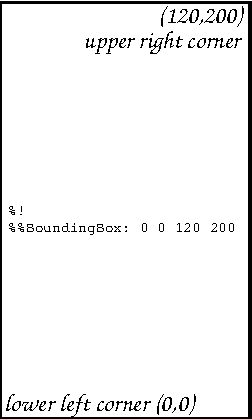
\includegraphics[width = 8.85cm]{fig1}
%\end{figure}

\begin{figure}
\caption{Meshed ``bare silicon" COMSOL model. Close up of finely meshed area near beam incidence is shown.}
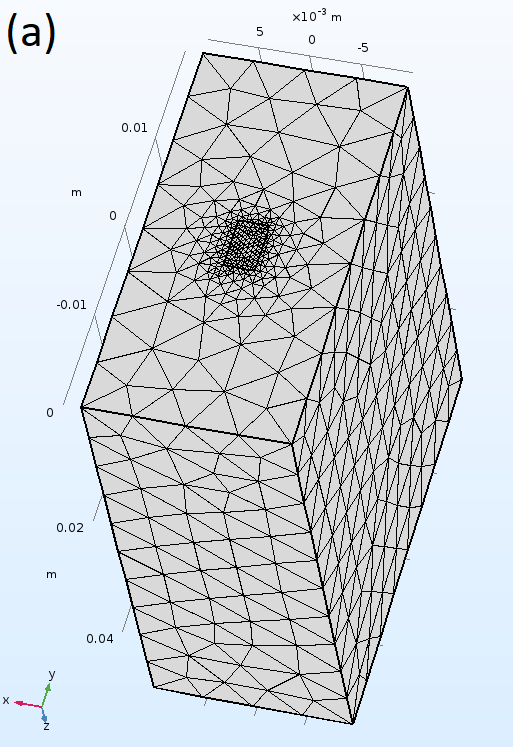
\includegraphics[width = 8.85cm]{images/bare_silicon.png}
\label{fig:bare_silicon}
\end{figure}


\begin{figure}
\caption{Image of physical SSRL model courtesy of Reference \cite{stanford}. Large reflective area and 4 large cut-outs for clamping seen. 14 through holes for liquid nitrogen are present on crystal sides.}
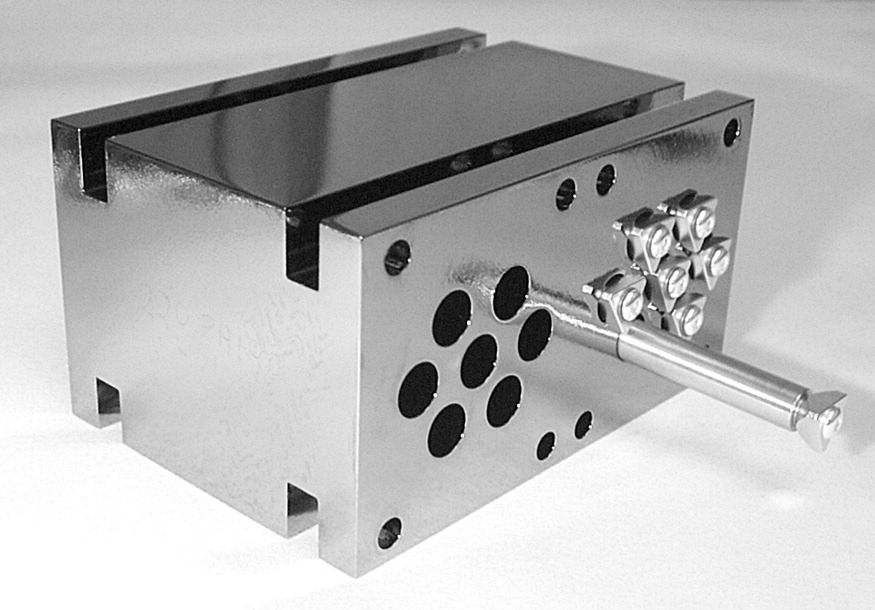
\includegraphics[width = 8.85cm]{images/ssrlsilicon.jpg}
\label{fig:ssrl_silicon}
\end{figure}


%\begin{figure}
%\caption{Unmeshed COMSOL model of the NanoMAX monochromator. \textbf{(a)} finely meshed beam incidence area, \textbf{(b)} %silicon crystal body, \textbf{(c)} copper cooling blocks, \textbf{(d)} nitrogen filled copper cooling pipes brazed to %cooling block bodies}
%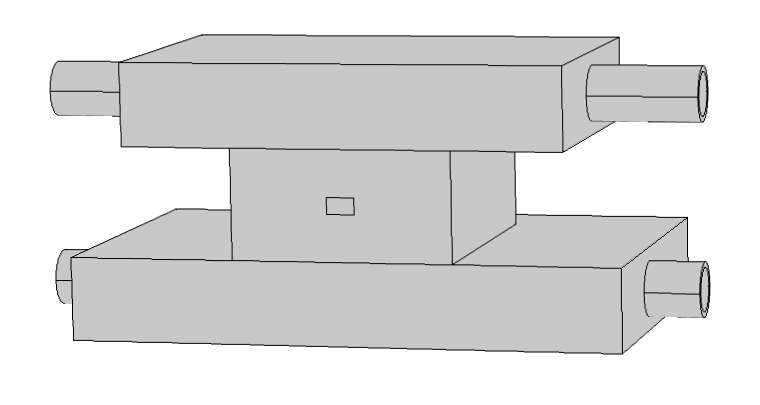
\includegraphics[width = 8.85cm]{images/nanomaxcomsol.png}
%\label{fig:nanomaxcomsol}
%\end{figure}


%\begin{figure}
%\caption{Diagram of beamline setup for Gaussian source simulations. From left to right are the X-ray source, the first crystal and the second. Absolute and relative distances are given in cm.}
%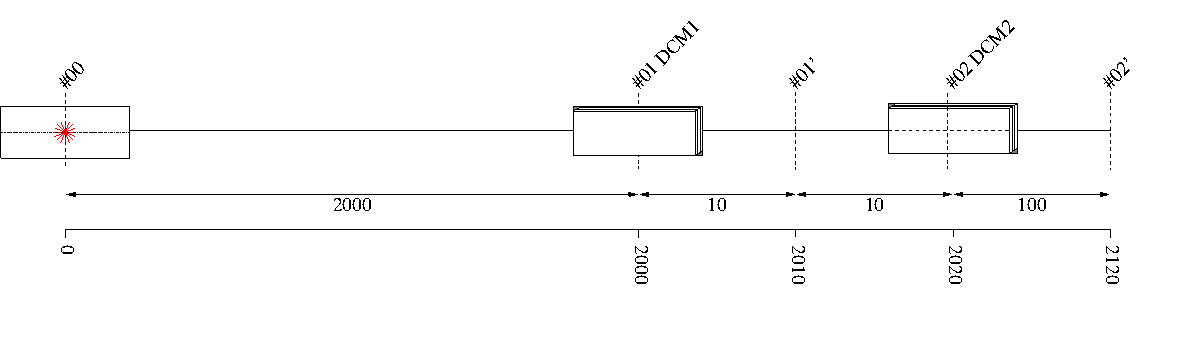
\includegraphics[width =8.85cm]{images/gaussian_beamline.png}
%\label{fig:dcmtracing}
%\end{figure}

\begin{table}\label{gaussian_table}
\caption{Gaussian beam parameters}
\begin{tabular}{@{}llll@{}}
Parameter       & Value         & Units     & Description                                           \\
\hline
x               & 0.005         & cm        & Gaussian $\sigma$ of horizontal irradiance            \\
z               & 0.0005        & cm        & Gaussian $\sigma$ of vertical irradiance              \\ 
y               & 0.0005        & cm        & Gaussian $\sigma$ of longitudinal irradiance          \\
x'              & 50            & mrad      & Gaussian $\sigma$ of horizontal angular intensity     \\
z'              & 50            & mrad      & Gaussian $\sigma$ of vertical angular intensity       \\

\end{tabular}
\end{table}

\begin{table}\label{ivubiomax}
\caption{Undulator Parameters}
\begin{tabular}{@{}llll@{}}
Parameter       & Value         & Units     & Description                           \\
\hline
$\lambda$       & 1.7           & cm              & magnetic period length                \\
n               & 176           & 1               & number of magnetic periods            \\ 
$l$             & 3             & m               & magnetic length                       \\
$K$             & 1.82          & 1               & max K value                           \\
$\sigma_x$      & 54            & $\mu$m          & electron beam horizontal rms size     \\
$\sigma_z$      & 4             & $\mu$m          & electron beam vertical rms size       \\
$\epsilon_x$    & 3.2e-08       & cm$\cdot$rad    & electron beam horizontal emittance    \\
$\epsilon_z$    & 8e-10         & cm$\cdot$rad    & electron beam vertical emittance      \\
I               & 500           & mA              & electron beam current                 \\
E               & 3             & GeV             & electron energy                       \\
\end{tabular}
\end{table}

\begin{table}\label{ivwbalder}
\caption{Wiggler Parameters}
\begin{tabular}{@{}llll@{}}
Parameter       & Value         & Units     & Description                           \\
\hline
$\lambda$       & 5             & cm        & magnetic period length                \\
n               & 40            & 1         & number of magnetic periods            \\ 
$l$             & 2             & m         & magnetic length                       \\
$K$             & 9             & 1         & max K value                           \\
$\sigma_x$      & 50            & $\mu$m    & electron beam horizontal rms size     \\
$\sigma_z$      & 2             & $\mu$m    & electron beam vertical rms size       \\
$\epsilon_x$    & 3.3e-08       & cm$\cdot$rad    & electron beam horizontal emittance    \\
$\epsilon_z$    & 8e-10         & cm$\cdot$rad    & electron beam vertical emittance      \\
I               & 500           & mA        & electron beam current                 \\
E               & 3             & GeV       & electron energy                       \\
\end{tabular}
\end{table}

\begin{comment}
\begin{figure}
\caption{Reflectively of 10~keV \textbf{(a)}, \textbf{(b)}, and 20~keV \textbf{(c)}, \textbf{(d)}, photons over deviations from Bragg angle in Si~111 with uniform strain depth gradient values and max temperatures of \textbf{(a)} 1.84e-02, 133~K, \textbf{(b)}  1.27e-01, 168~K, \textbf{(c)} 1.84e-02, 133~K, and \textbf{(d)}  1.27e-01, 168~K}
\includegraphics[width =\textwidth]{images/111USG.png}
\label{fig:111USG}
\end{figure}
\begin{figure}
\caption{Rocking curve for an 8~keV photon in a Si~333 crystal with a USG of 0.02906~m$^{-1}$.}
\includegraphics[width = \textwidth]{images/333USG.png}
\label{fig:333USG}
\end{figure}
\end{comment}

\begin{figure}
\caption{20~keV photons over deviations from Bragg angle in Si~333 with uniform strain depth gradient value of 0.0225~m$^{-1}$}
\includegraphics[width = \textwidth]{images/333USG.png}
\label{fig:333USG}
\end{figure}

\begin{figure}

\caption{Charts of deformation and temperature along the center of the surface of silicon crystal in the meridional direction. Temperature is given by the green dashed line and deformation by the blue solid line. Max temperatures in the crystal are \textbf{(a)} 133~K, \textbf{(b)} 144~K, \textbf{(c)} 156~K, \textbf{(d)} 168~K, \textbf{(e)} 180~K, and \textbf{f)} 192~K. Charts generated from simulations performed in COMSOL.}
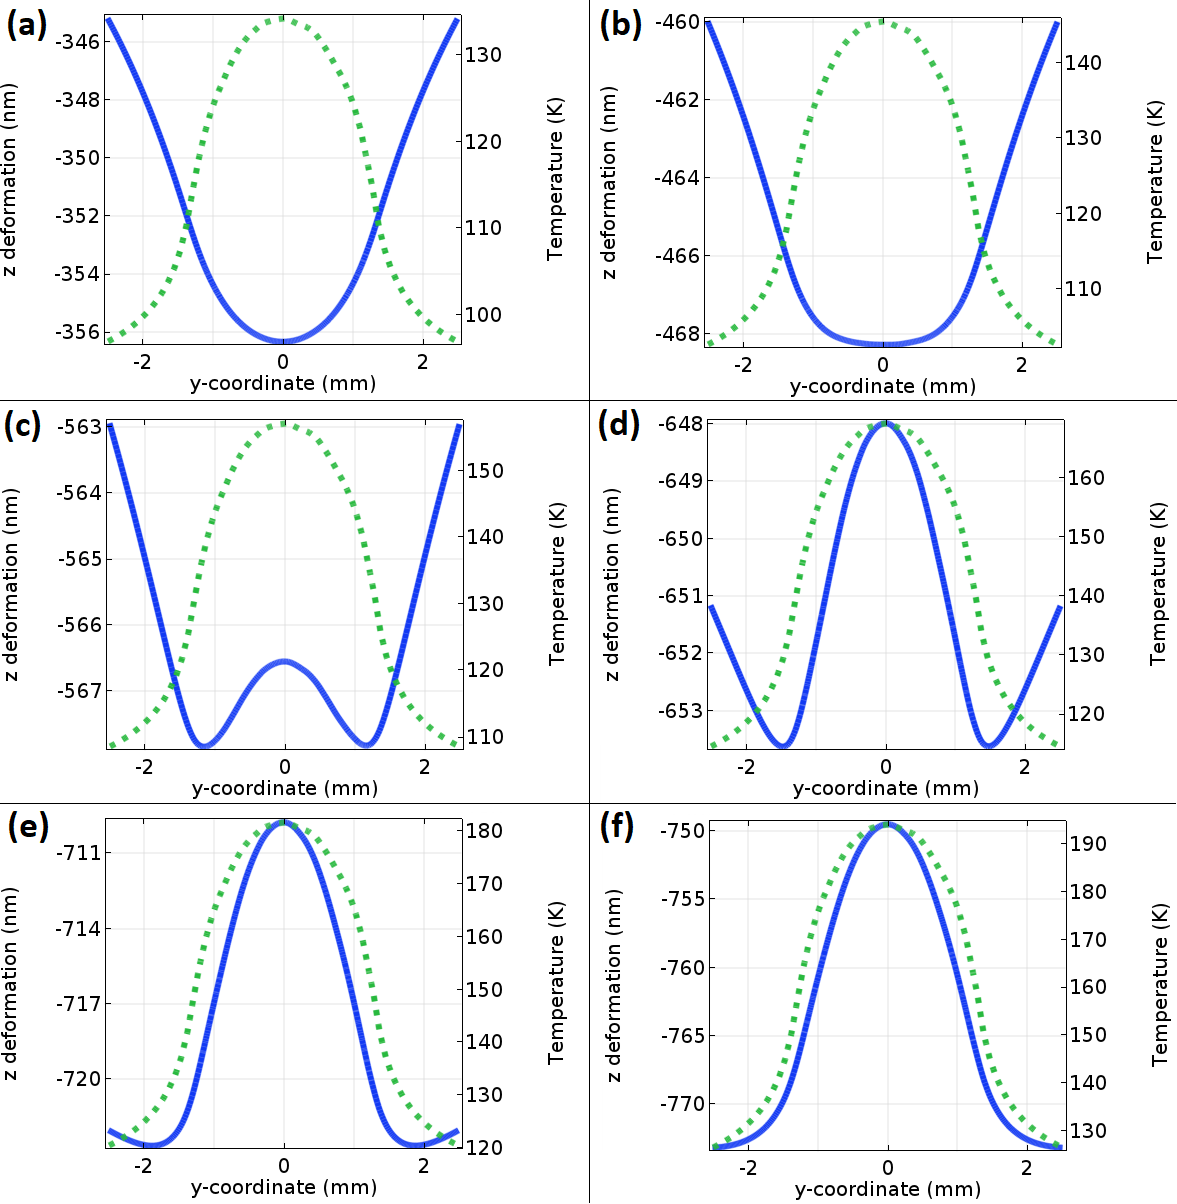
\includegraphics[width = \textwidth]{images/deformation.png}

\label{fig:ydeformation}
\end{figure}

\begin{figure}
\caption{Slope of error due to thermal buckling of 1st crystal in the meridional direction. Legend gives associated maximum temperature in the crystal.}
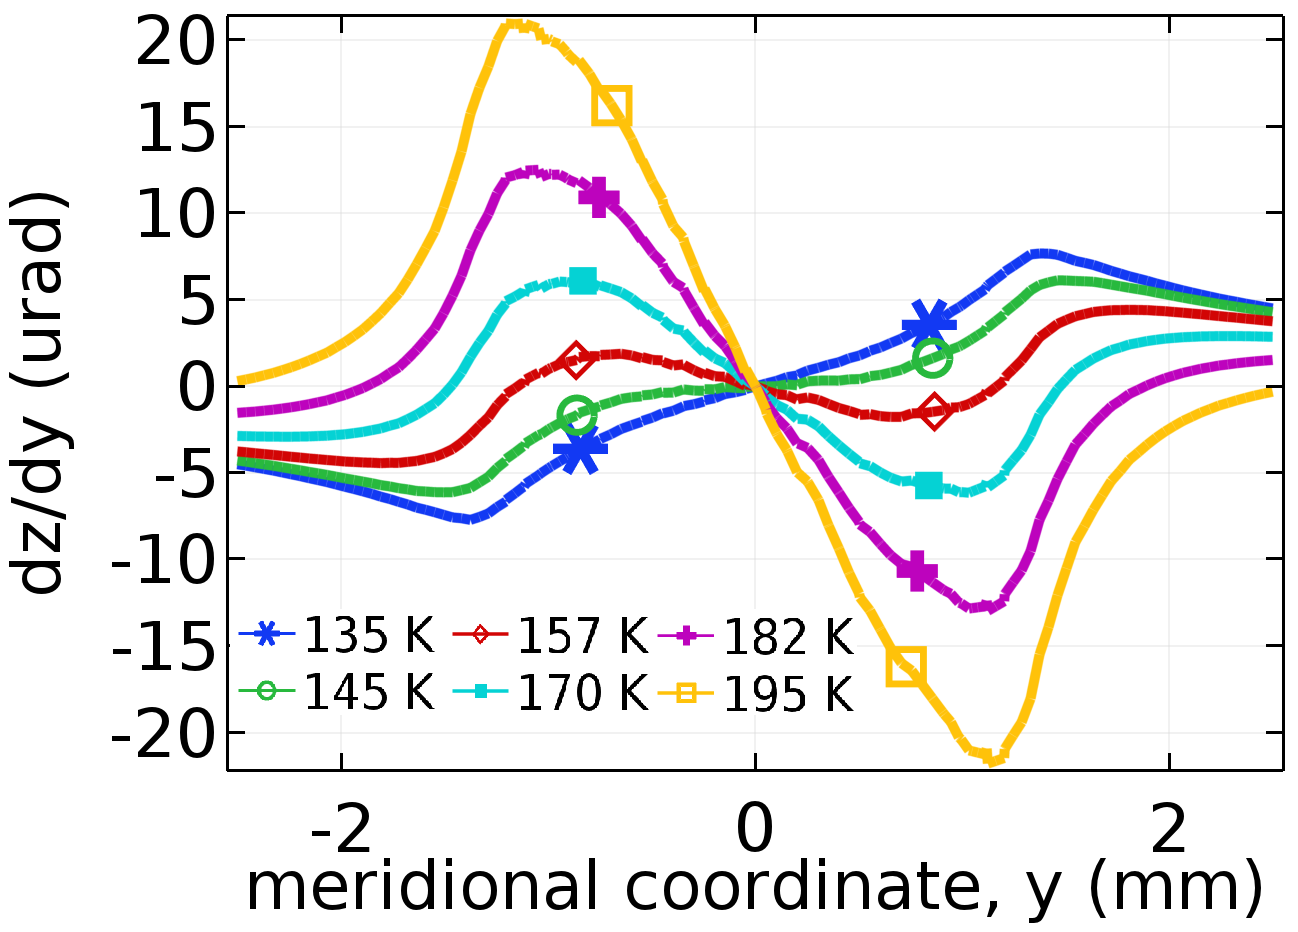
\includegraphics[width = 8.85cm]{images/slope.png}
\label{fig:yslope}
\end{figure}

\begin{figure}
\caption{Double crystal photon flux in Si~111 for strained and unstrained cases using a Gaussian source}
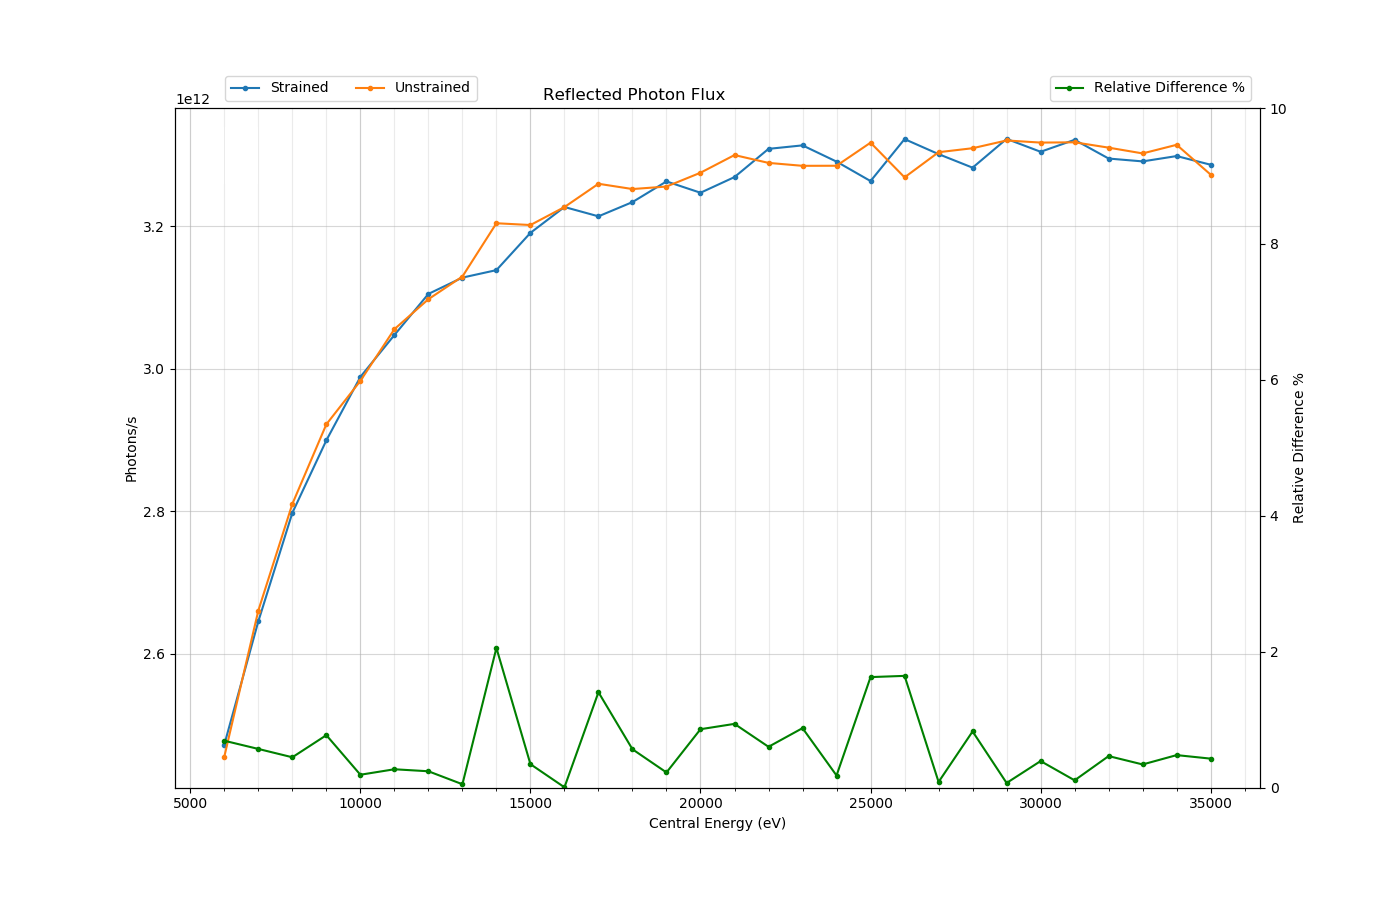
\includegraphics[width = 8.85cm]{images/111flux.png}
\label{fig:111flux}
\end{figure}

\begin{figure}
\caption{Double crystal monochromator bandwidth in Si~111 for strained and unstrained cases using a Gaussian source}
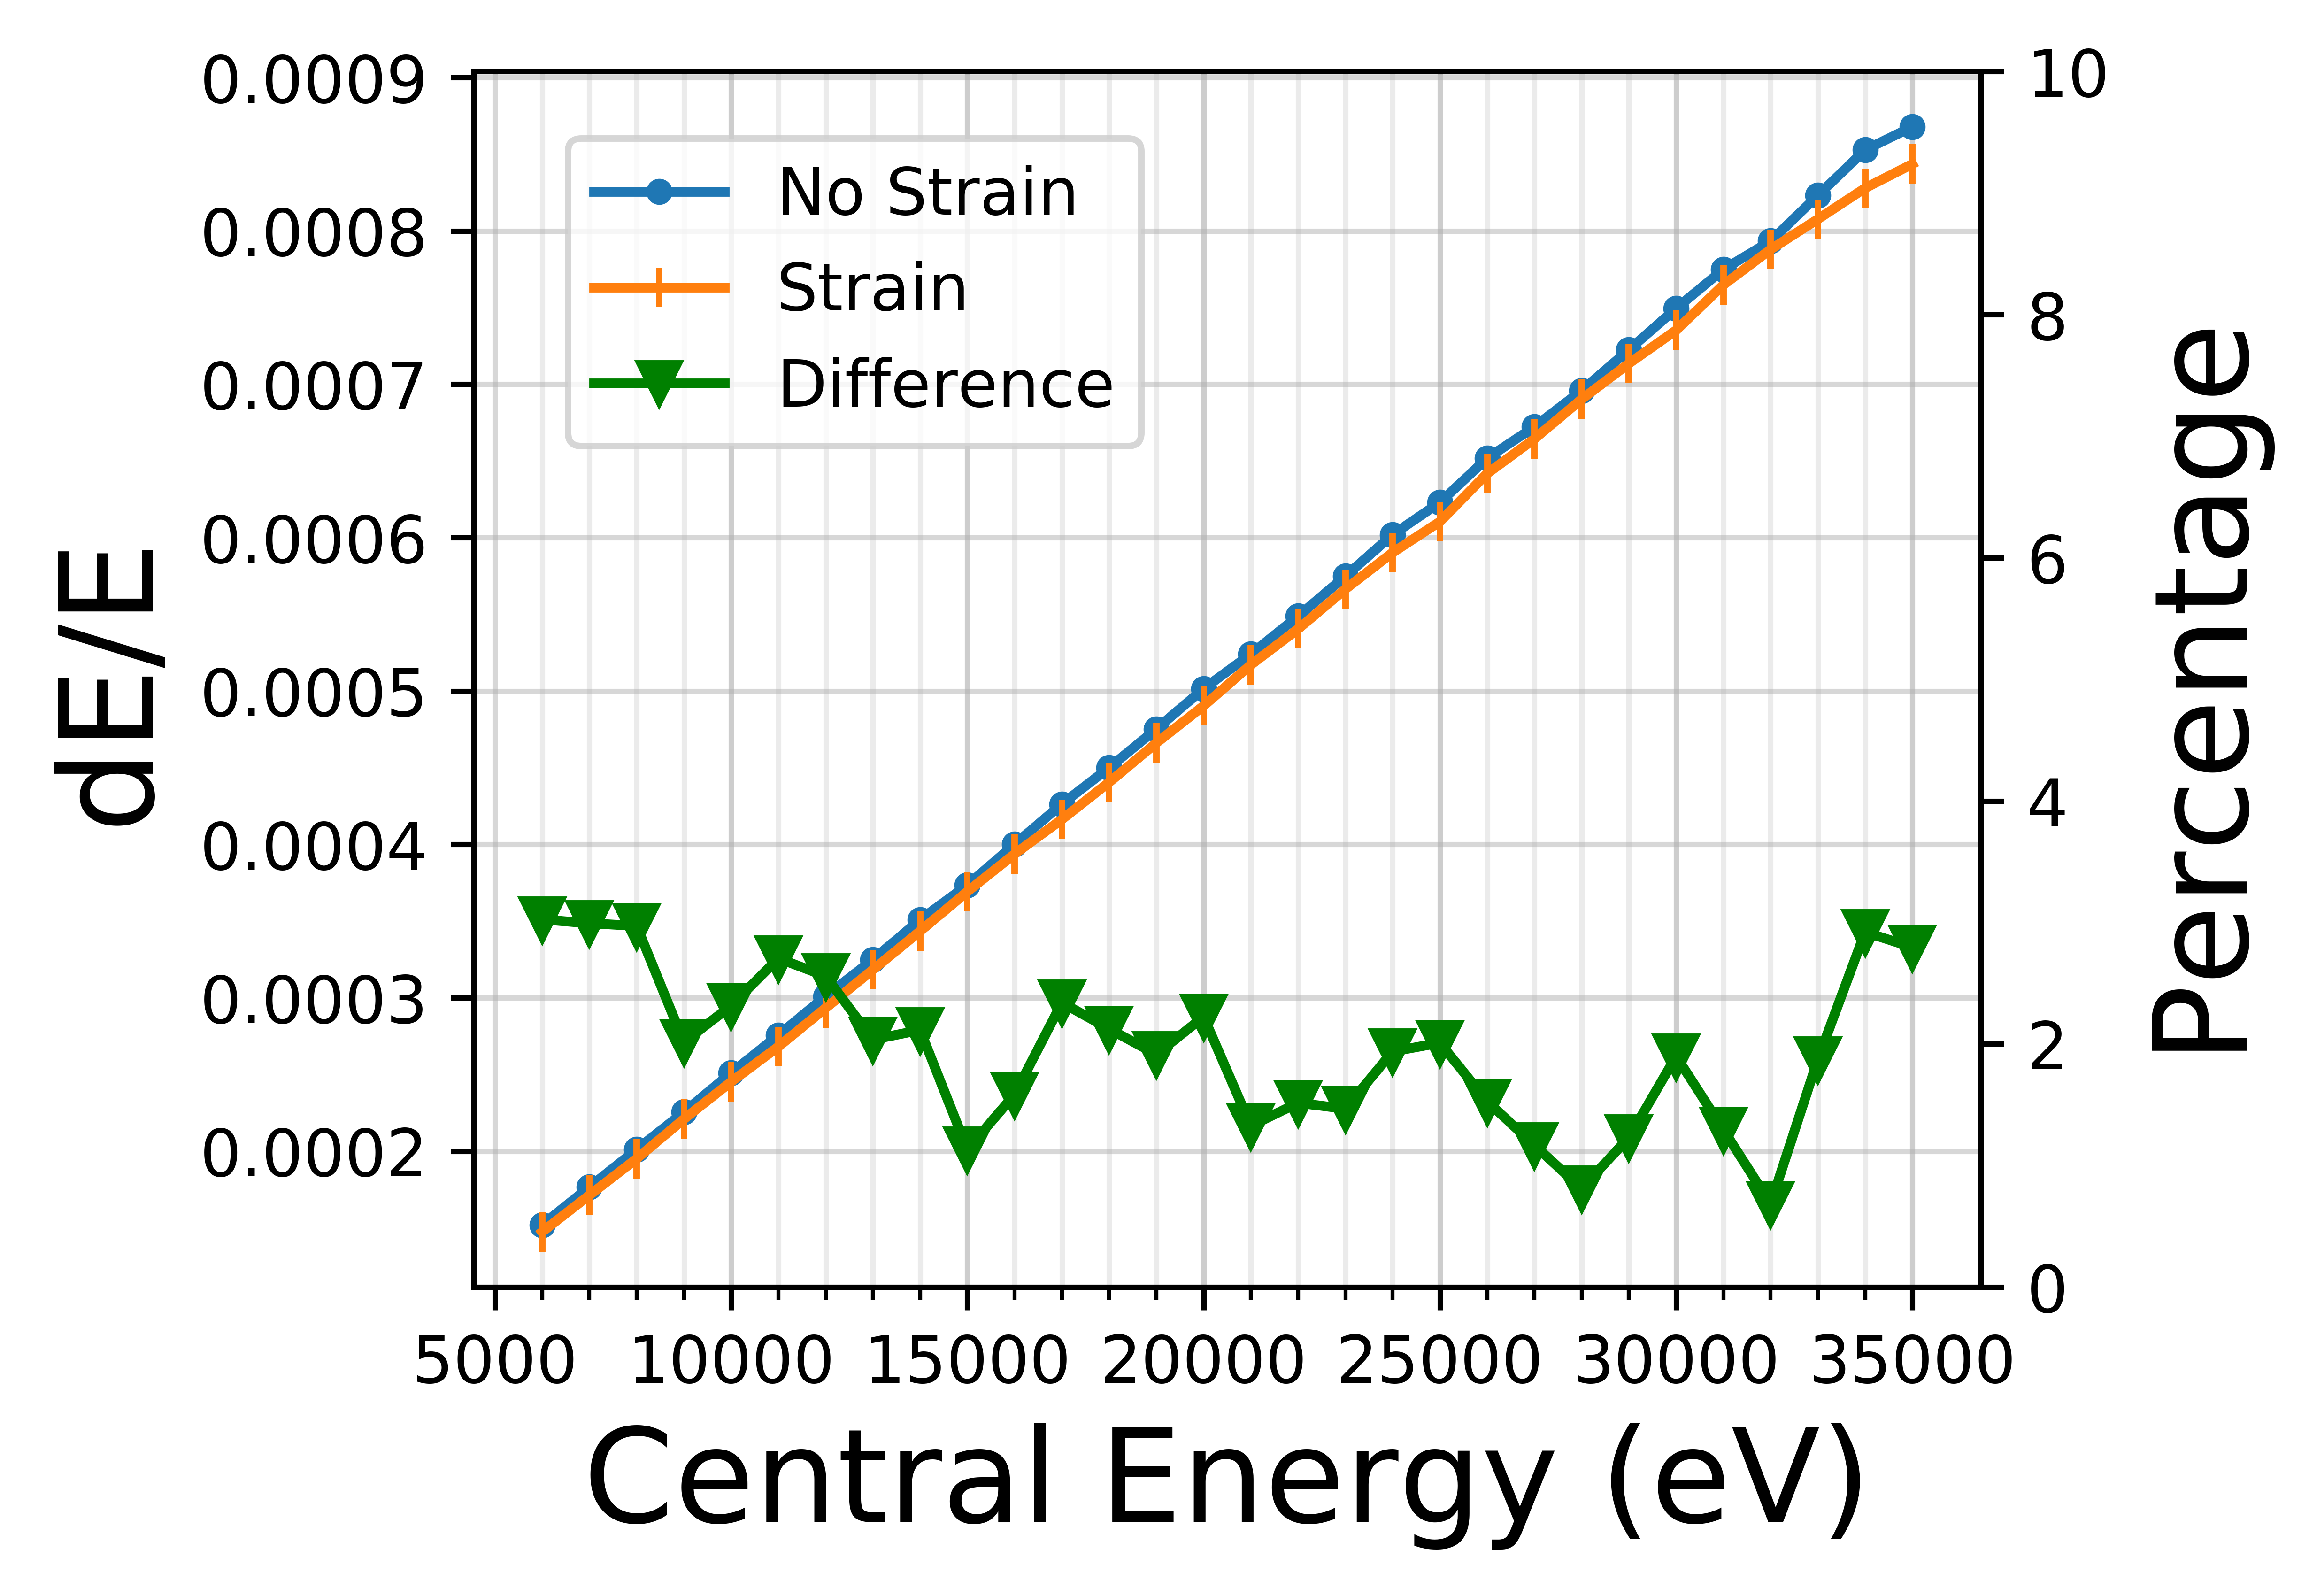
\includegraphics[width = 8.85cm]{images/111monobw.png}
\label{fig:111monobw}
\end{figure}

\begin{figure}
\caption{Double crystal photon flux in Si~333 for strained and unstrained cases using a Gaussian source}
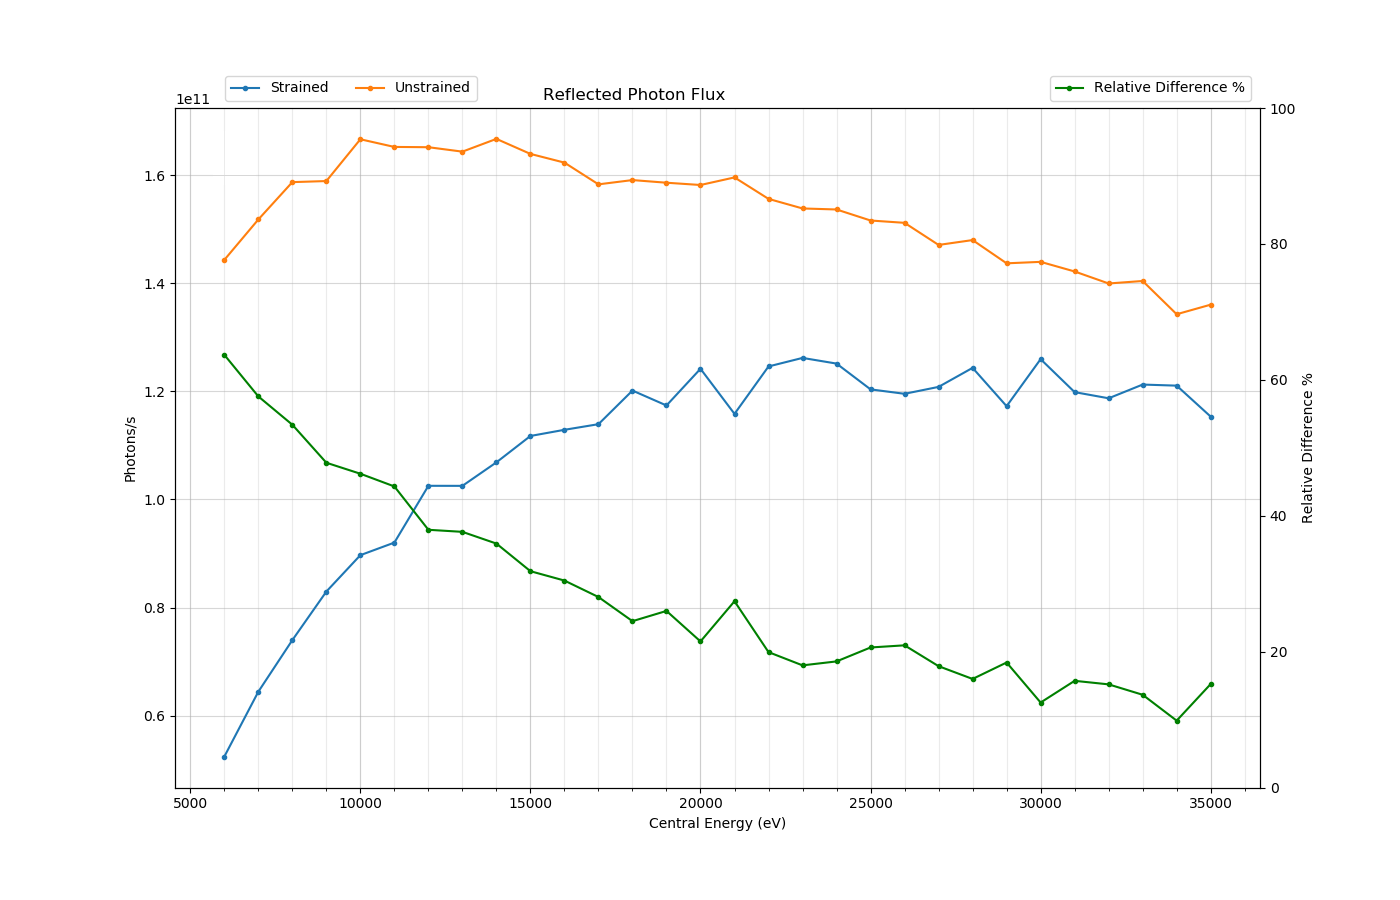
\includegraphics[width = 8.85cm]{images/333flux.png}
\label{fig:333flux}
\end{figure}

\begin{figure}
\caption{Double crystal monochromator bandwidth in Si~333 for strained and unstrained cases using a Gaussian source}
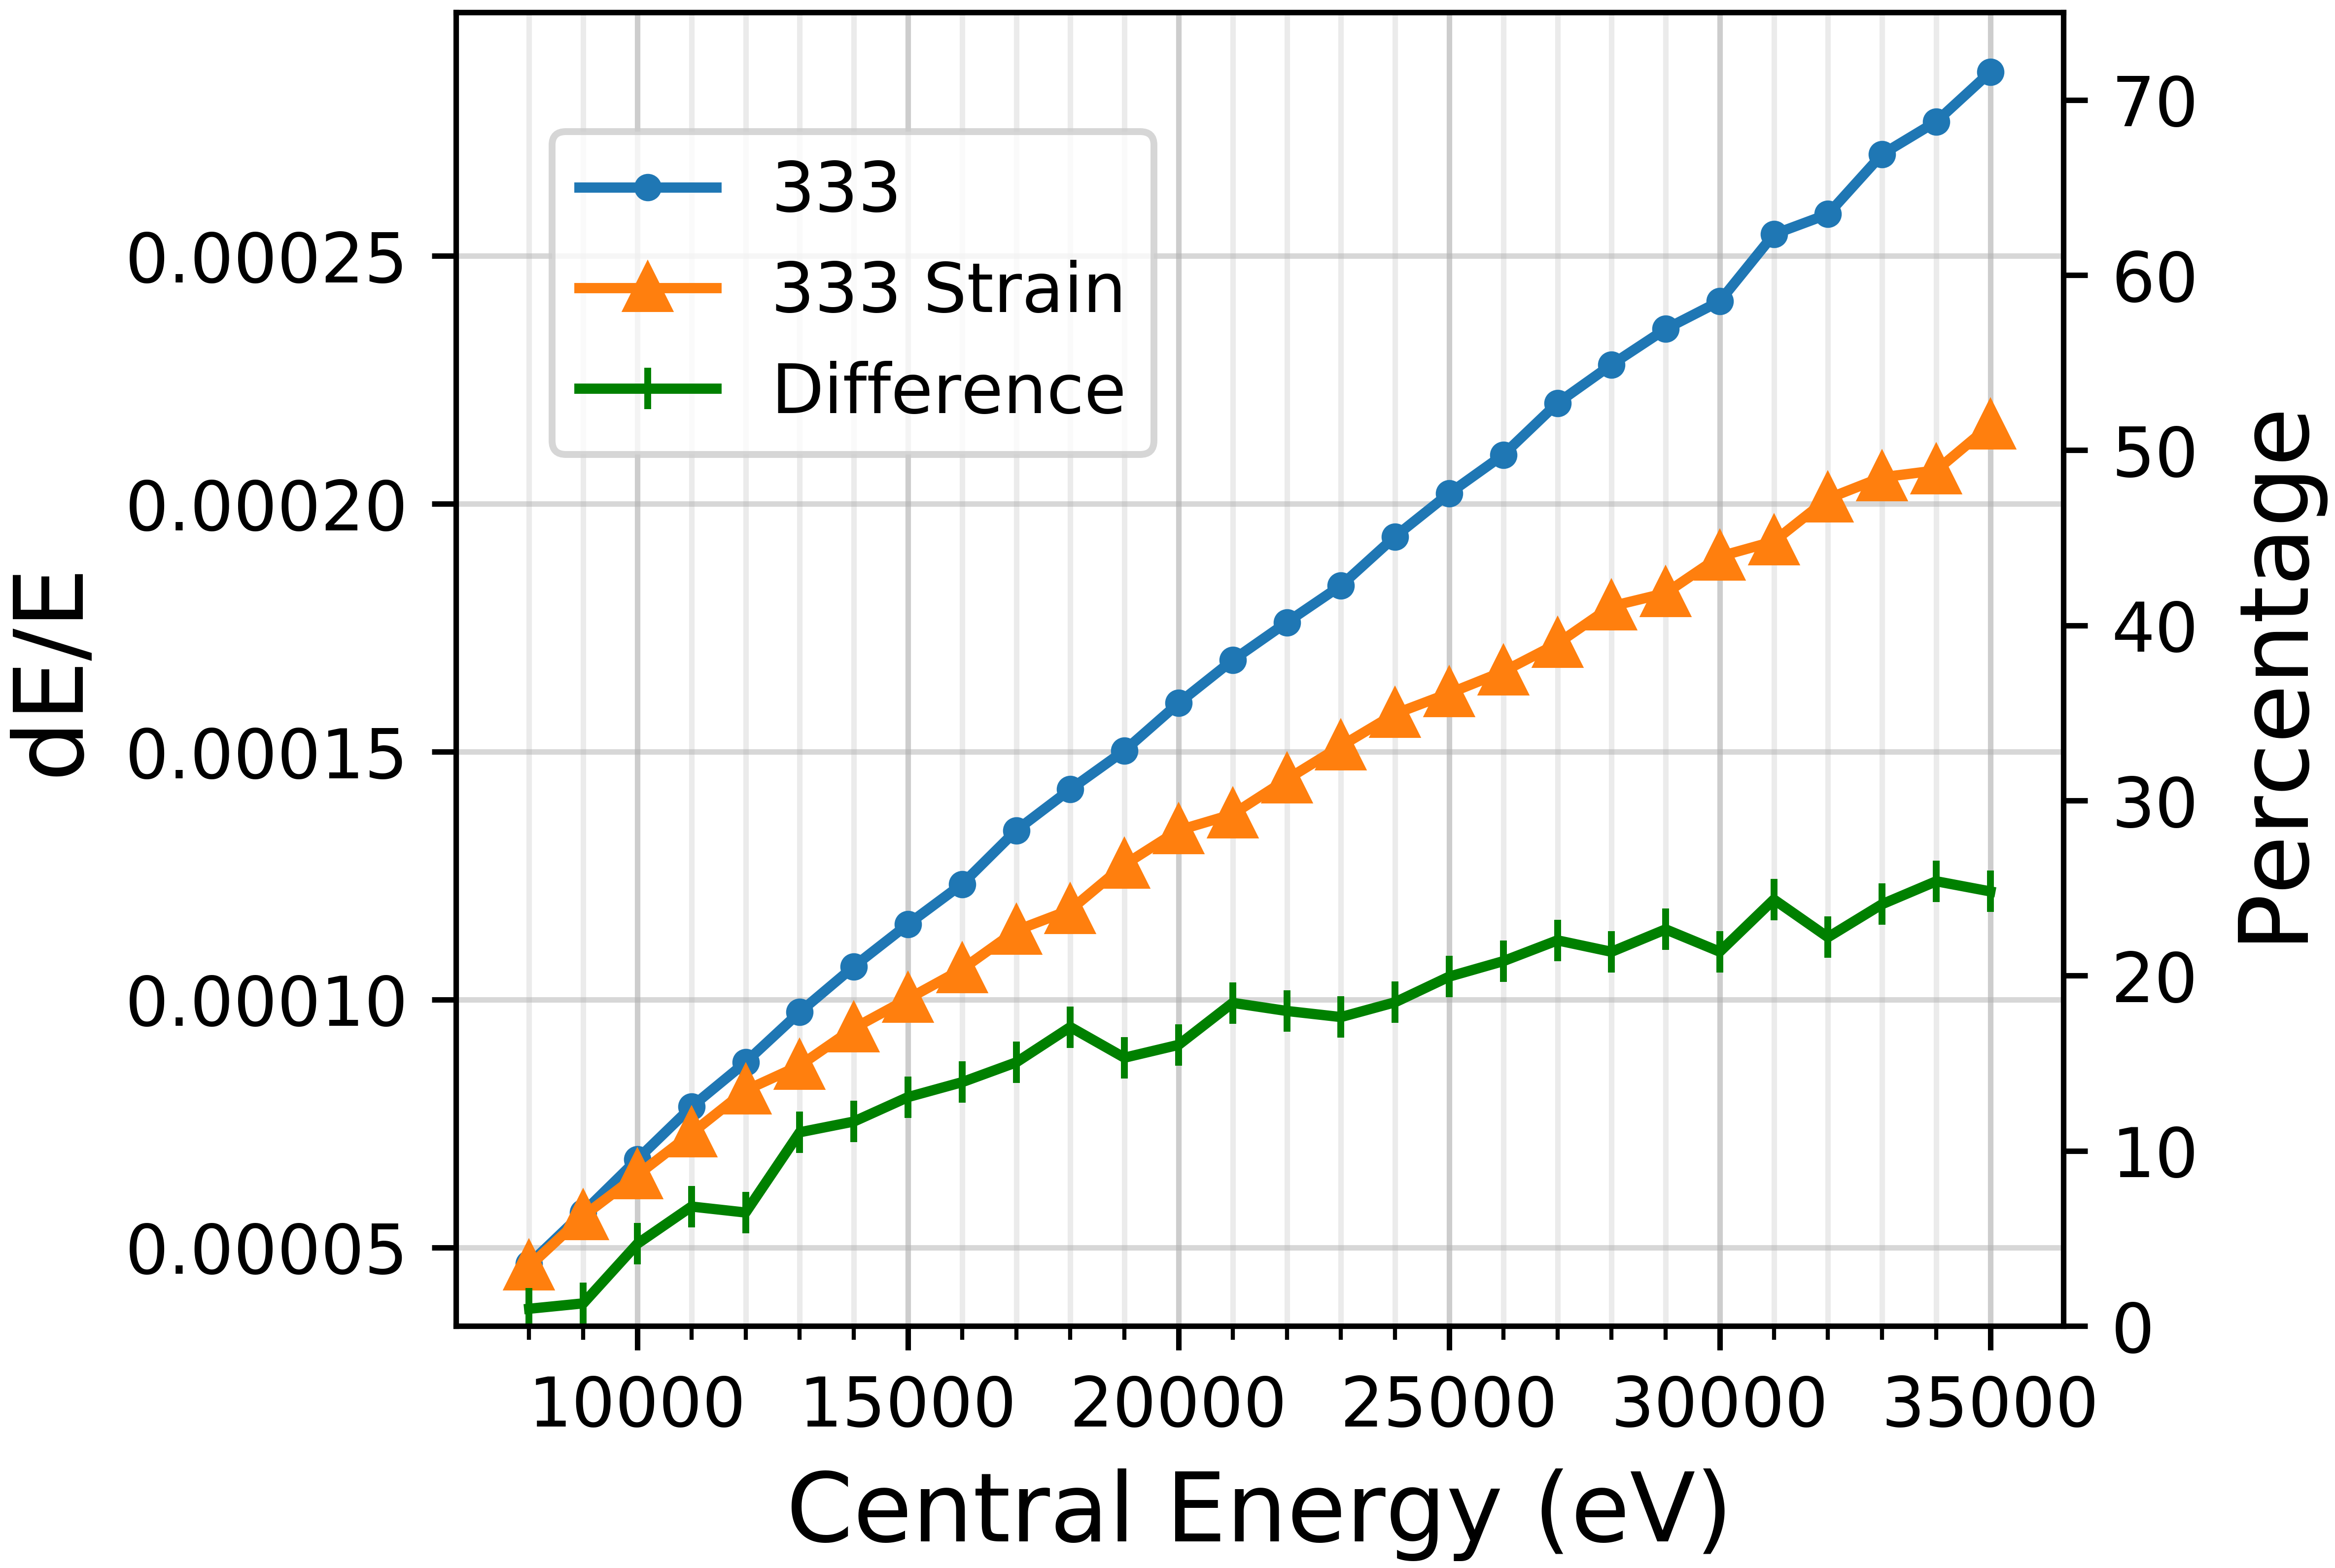
\includegraphics[width = 8.85cm]{images/333monobw.png}
\label{fig:333monobw}
\end{figure}

\begin{figure}
\caption{Double crystal photon flux in Si~333 for strained and unstrained cases using a Gaussian source. Source power is varied and stated by the legend in units of Watt. Photon flux is normalized to the 50~W case. The upper four lines are without strain while the bottom four includes it.}
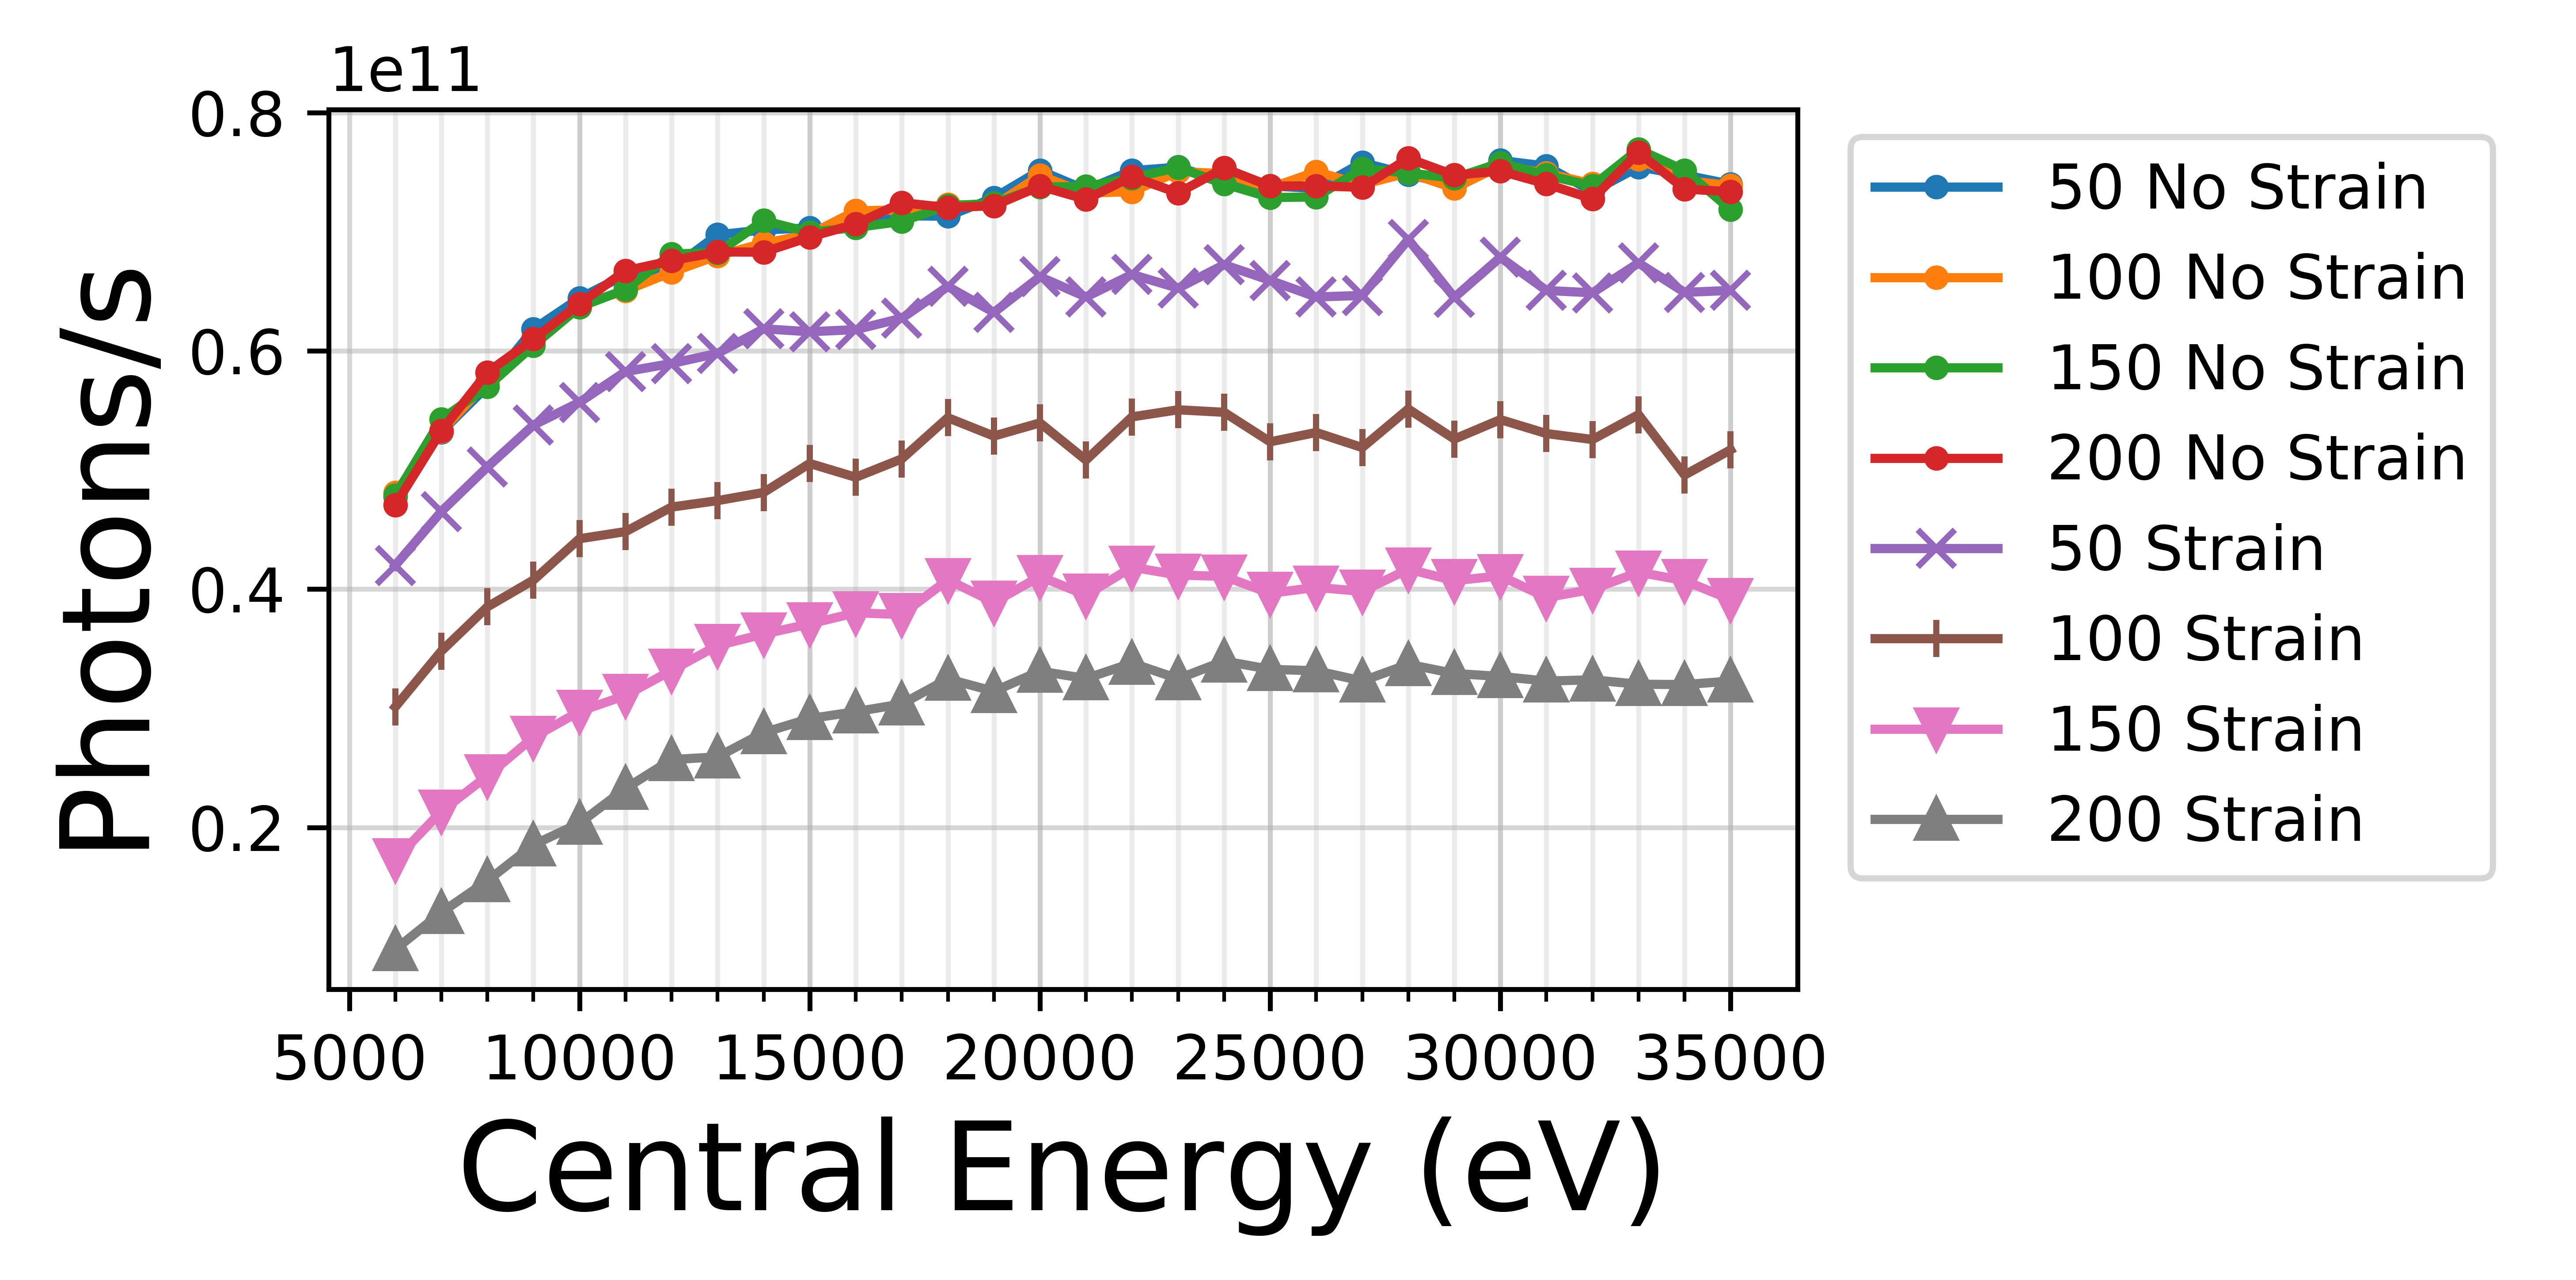
\includegraphics[width = 8.85cm]{images/333strainpower.png}
\label{fig:333strainpower}
\end{figure}

\begin{figure}
\caption{Double crystal photon flux in Si~333 for strained and unstrained cases using a Gaussian source. Source distance is varied and stated by the legend in units of meter. The upper four lines are without strain while the bottom four includes it.}
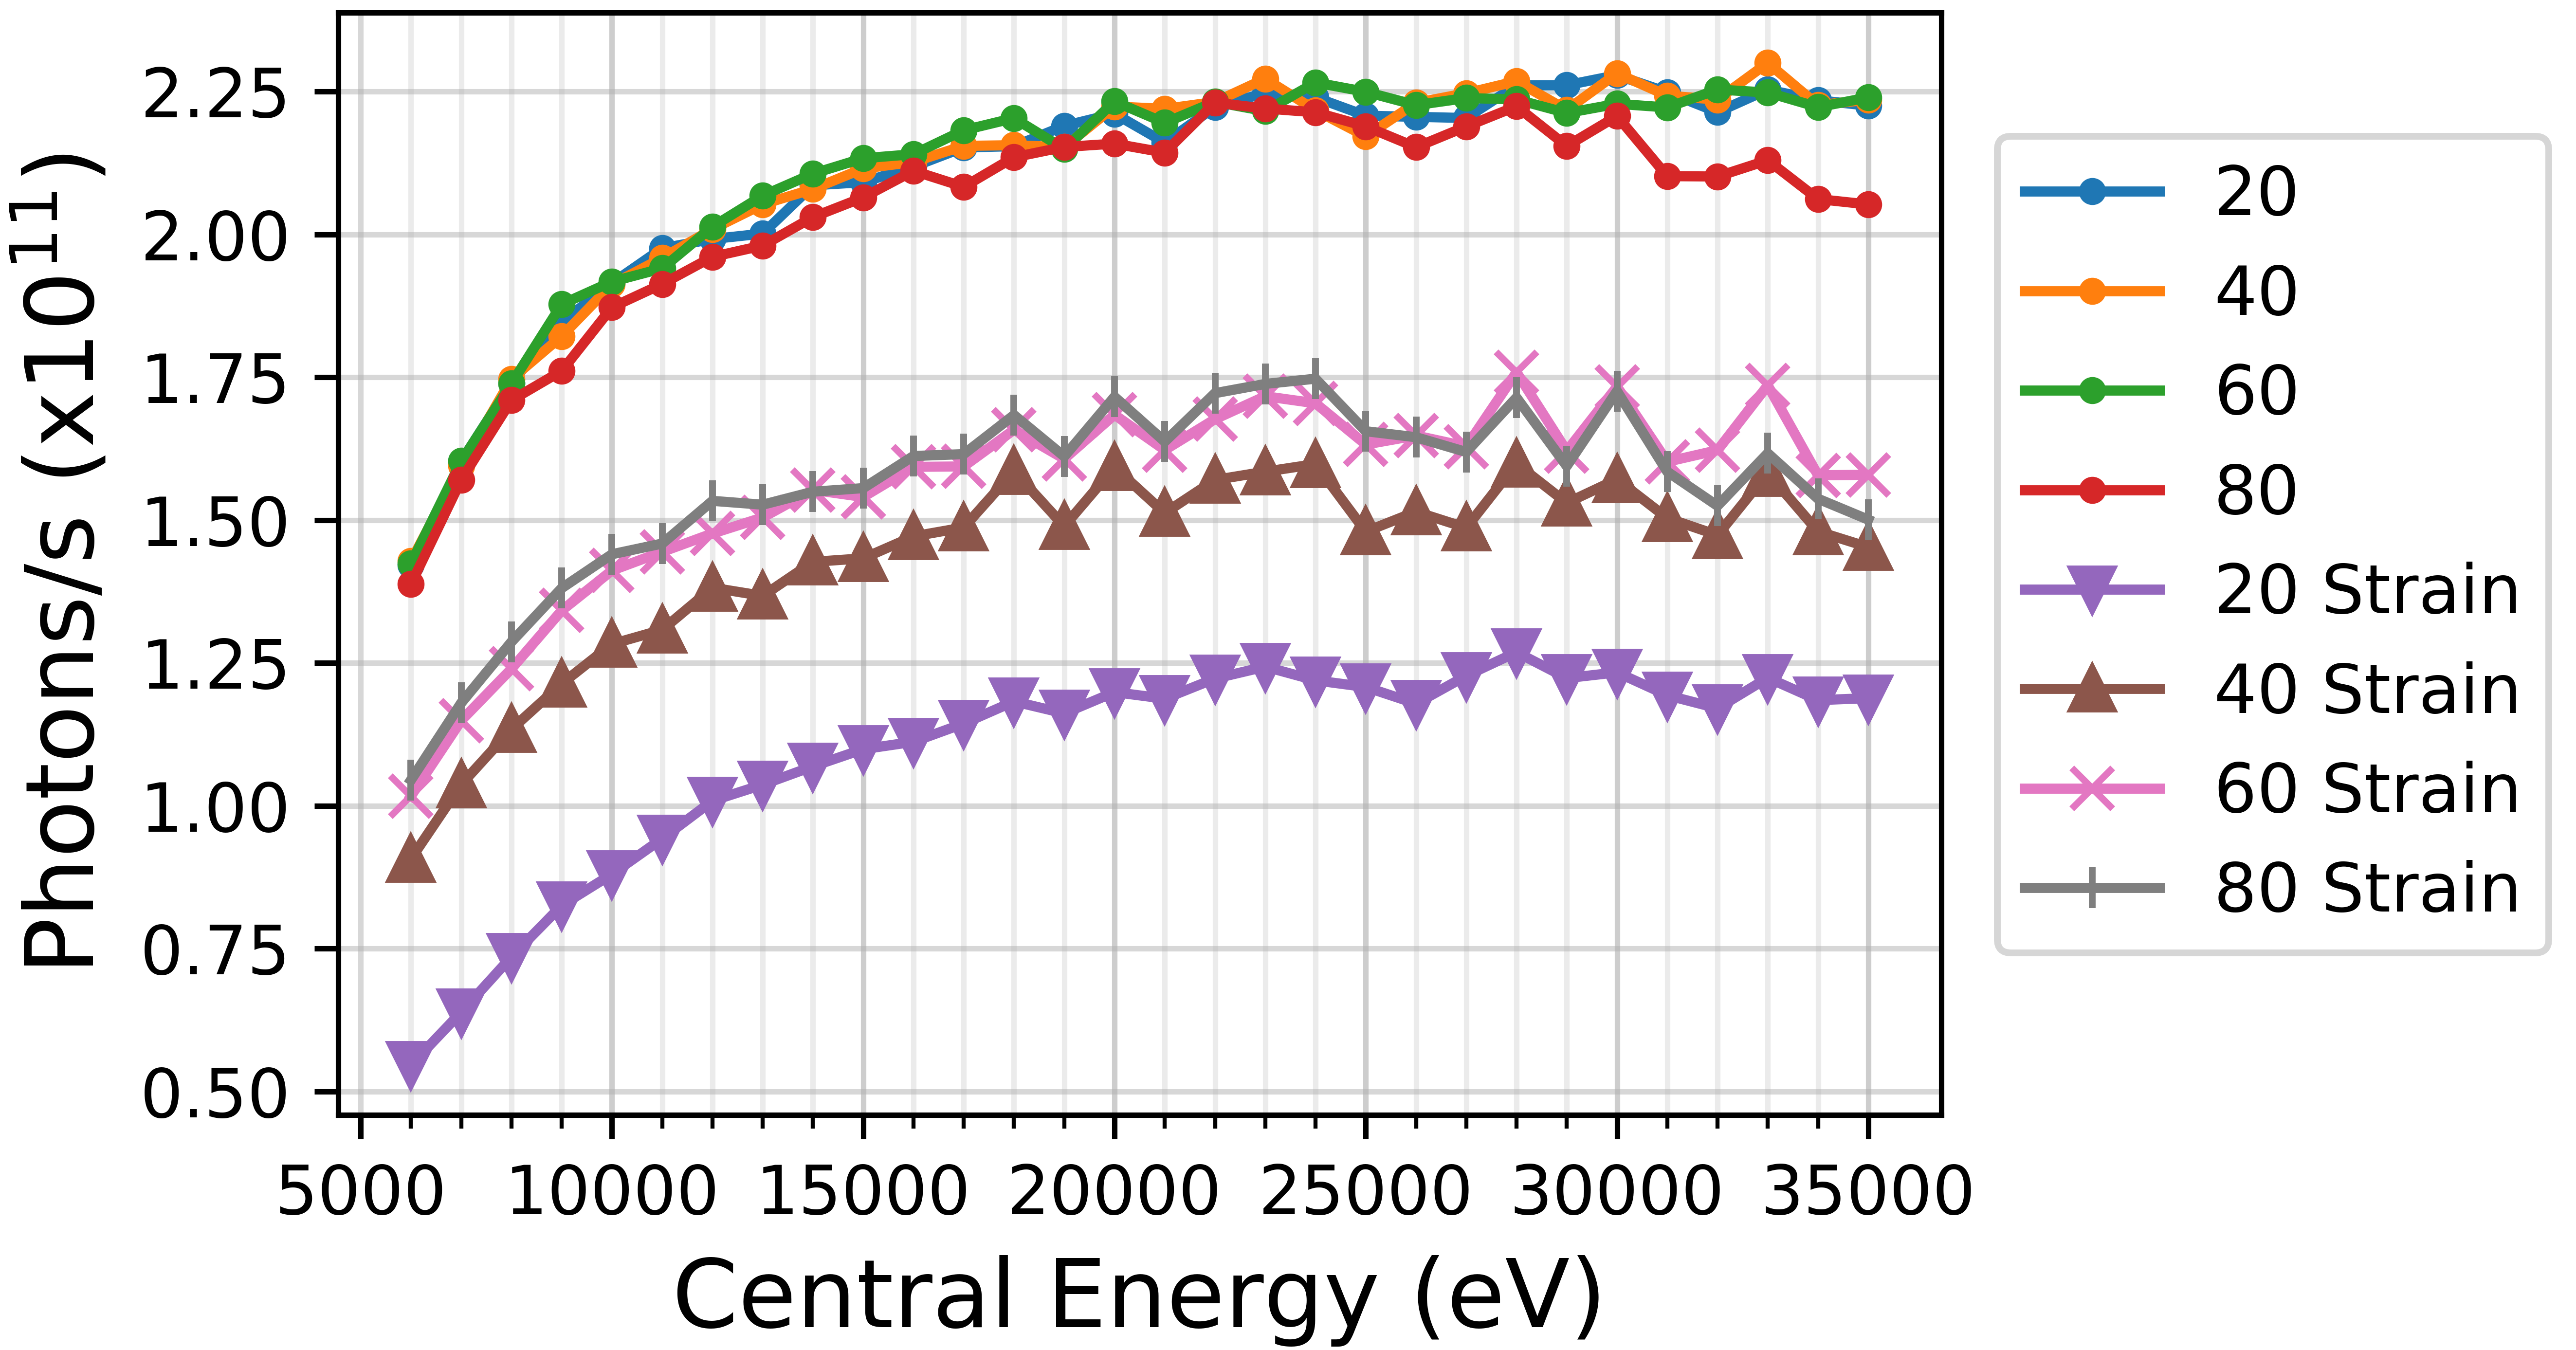
\includegraphics[width = 8.85cm]{images/333straindistance.png}
\label{fig:333straindistance}
\end{figure}

\begin{figure}
\caption{Double crystal photon flux in Si~333 for strained and unstrained cases using a Gaussian source. Source divergence is varied as (25,25), (50,50), (75,75), (100,100) units of mrad$^2$. Power per area on crystal surface is normalized to the 25$\times$25 mrad$^2$ case. The upper four lines are without strain while the bottom four includes it.}
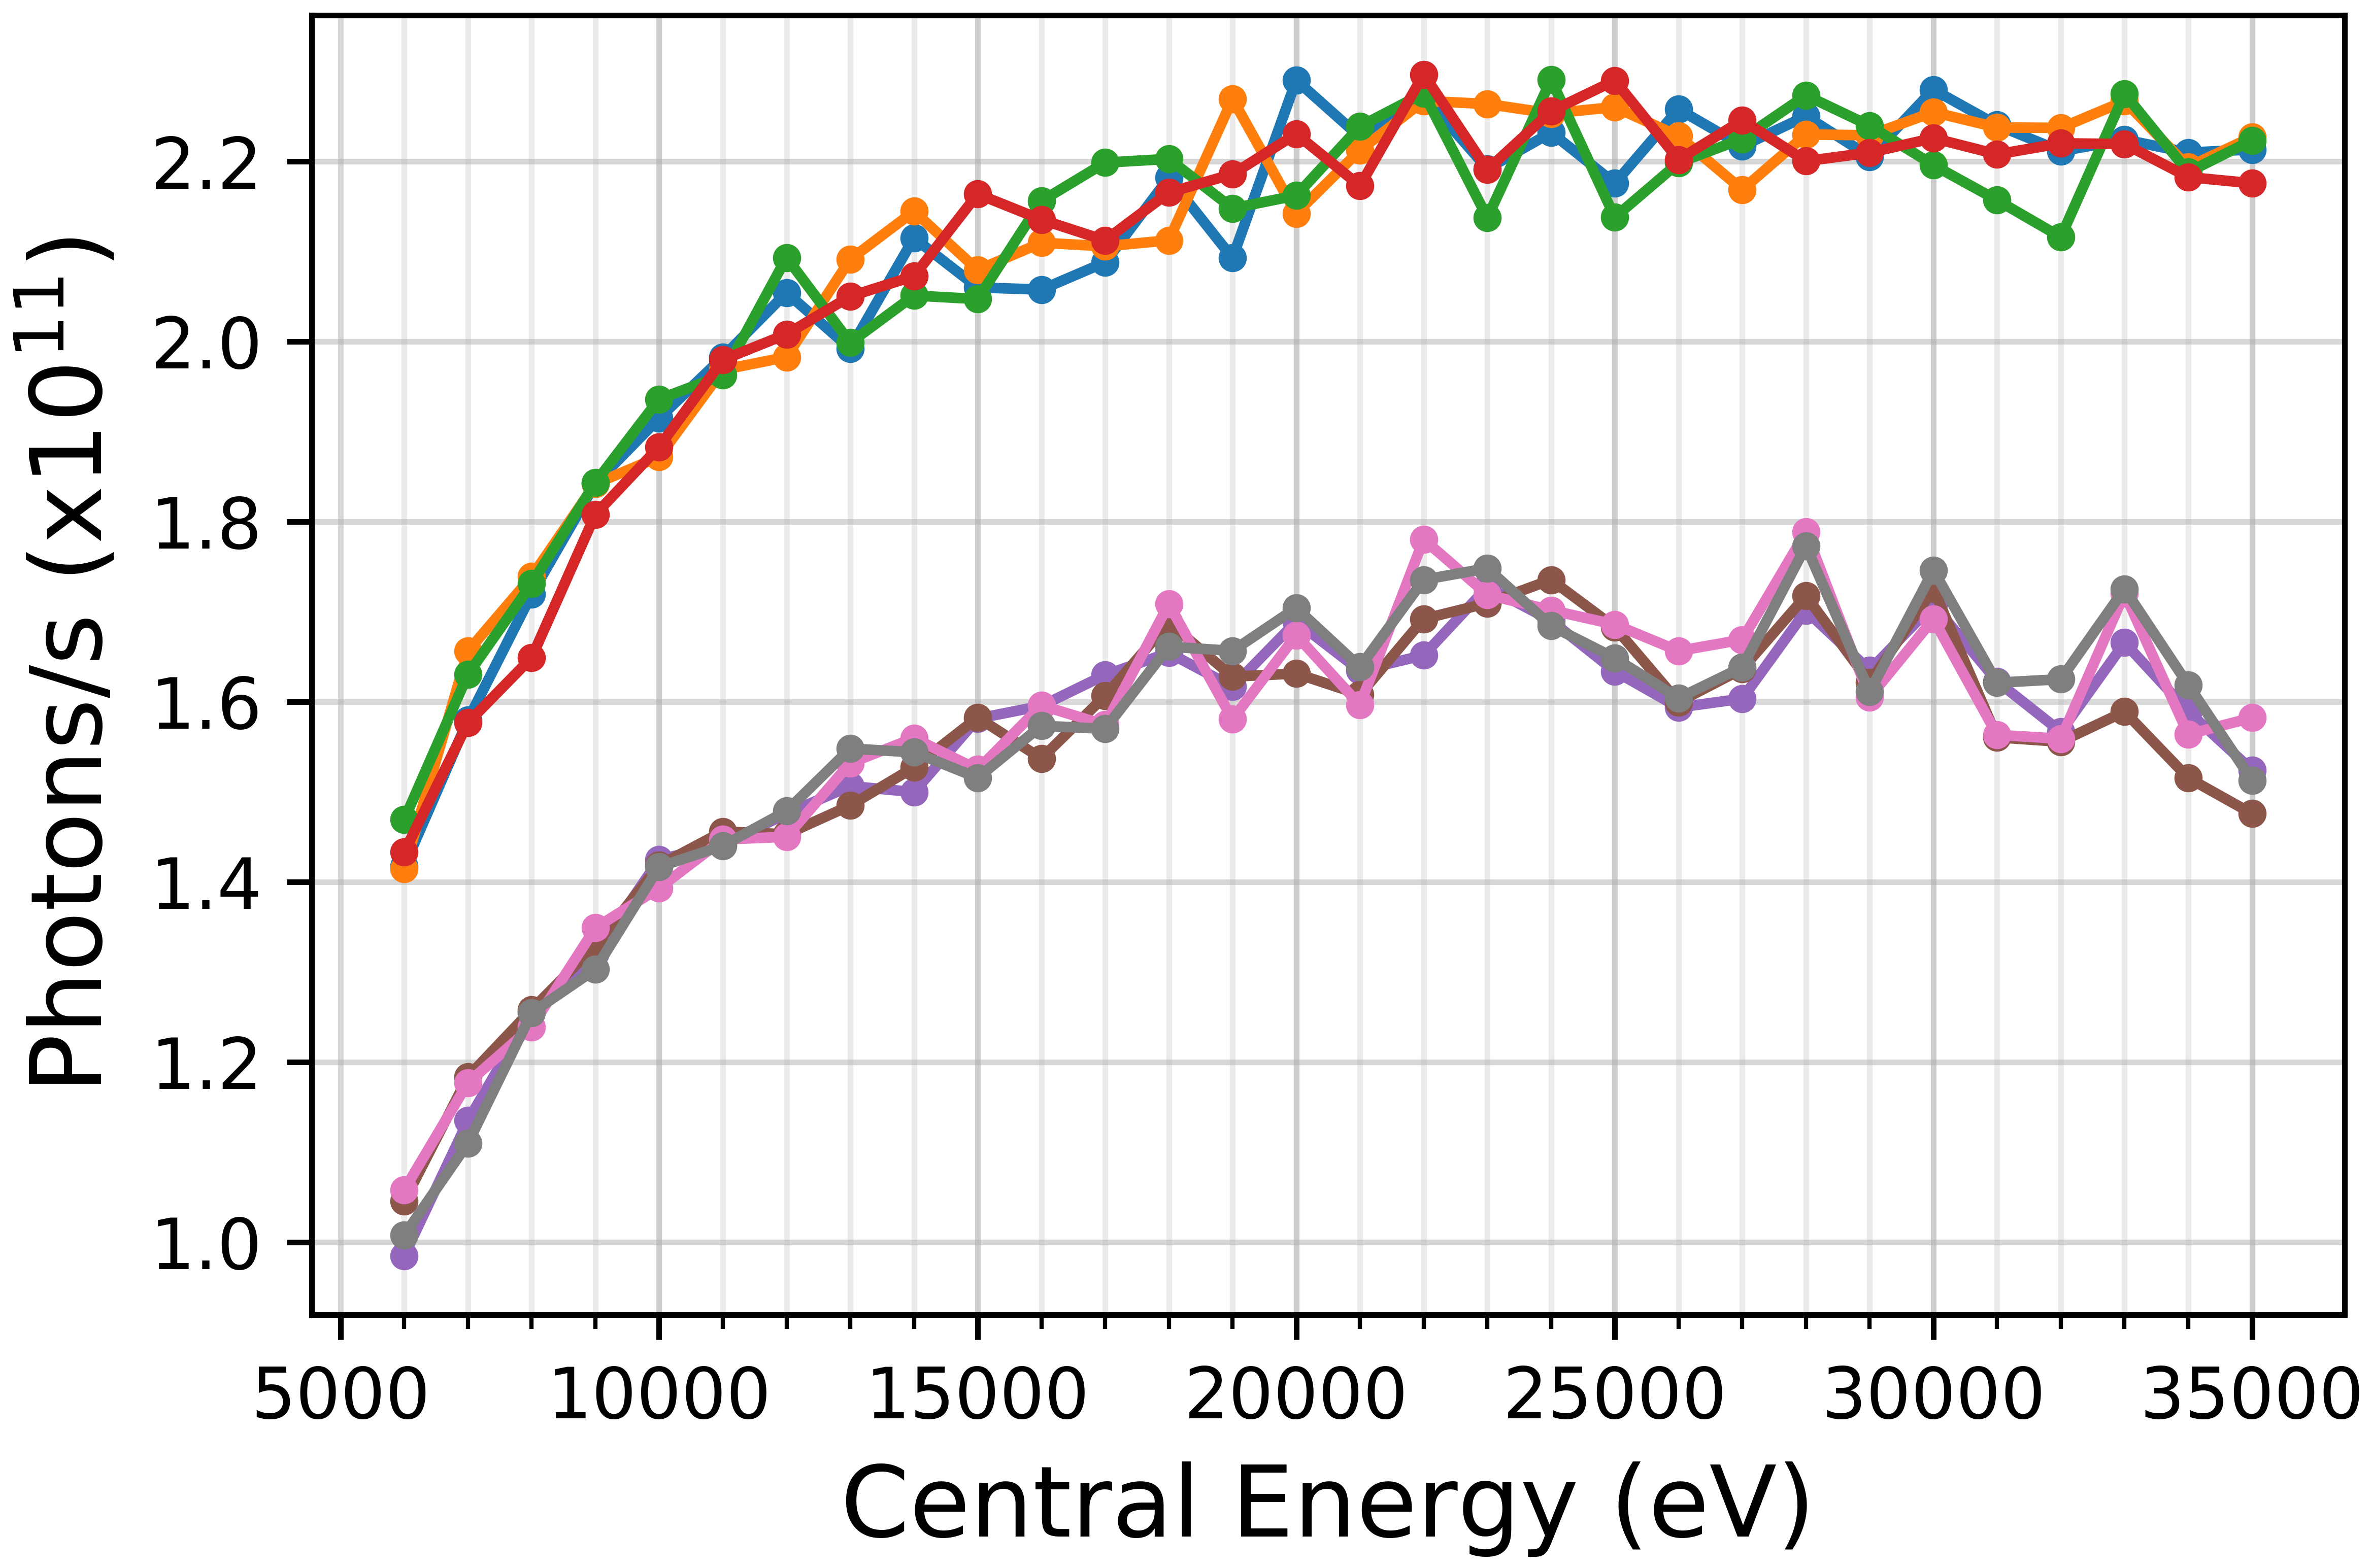
\includegraphics[width = 8.85cm]{images/333straindivergence.png}
\label{fig:333straindivergence}
\end{figure}

\begin{figure}
\caption{Double crystal photon flux in Si~333 for strained and unstrained cases using a Gaussian source. Source size is varied as (0,0), (25,2.5), (50,5.0), (75,7.5), and (100,10) in units of micron$^2$. The upper four lines are without strain while the bottom four includes it.}
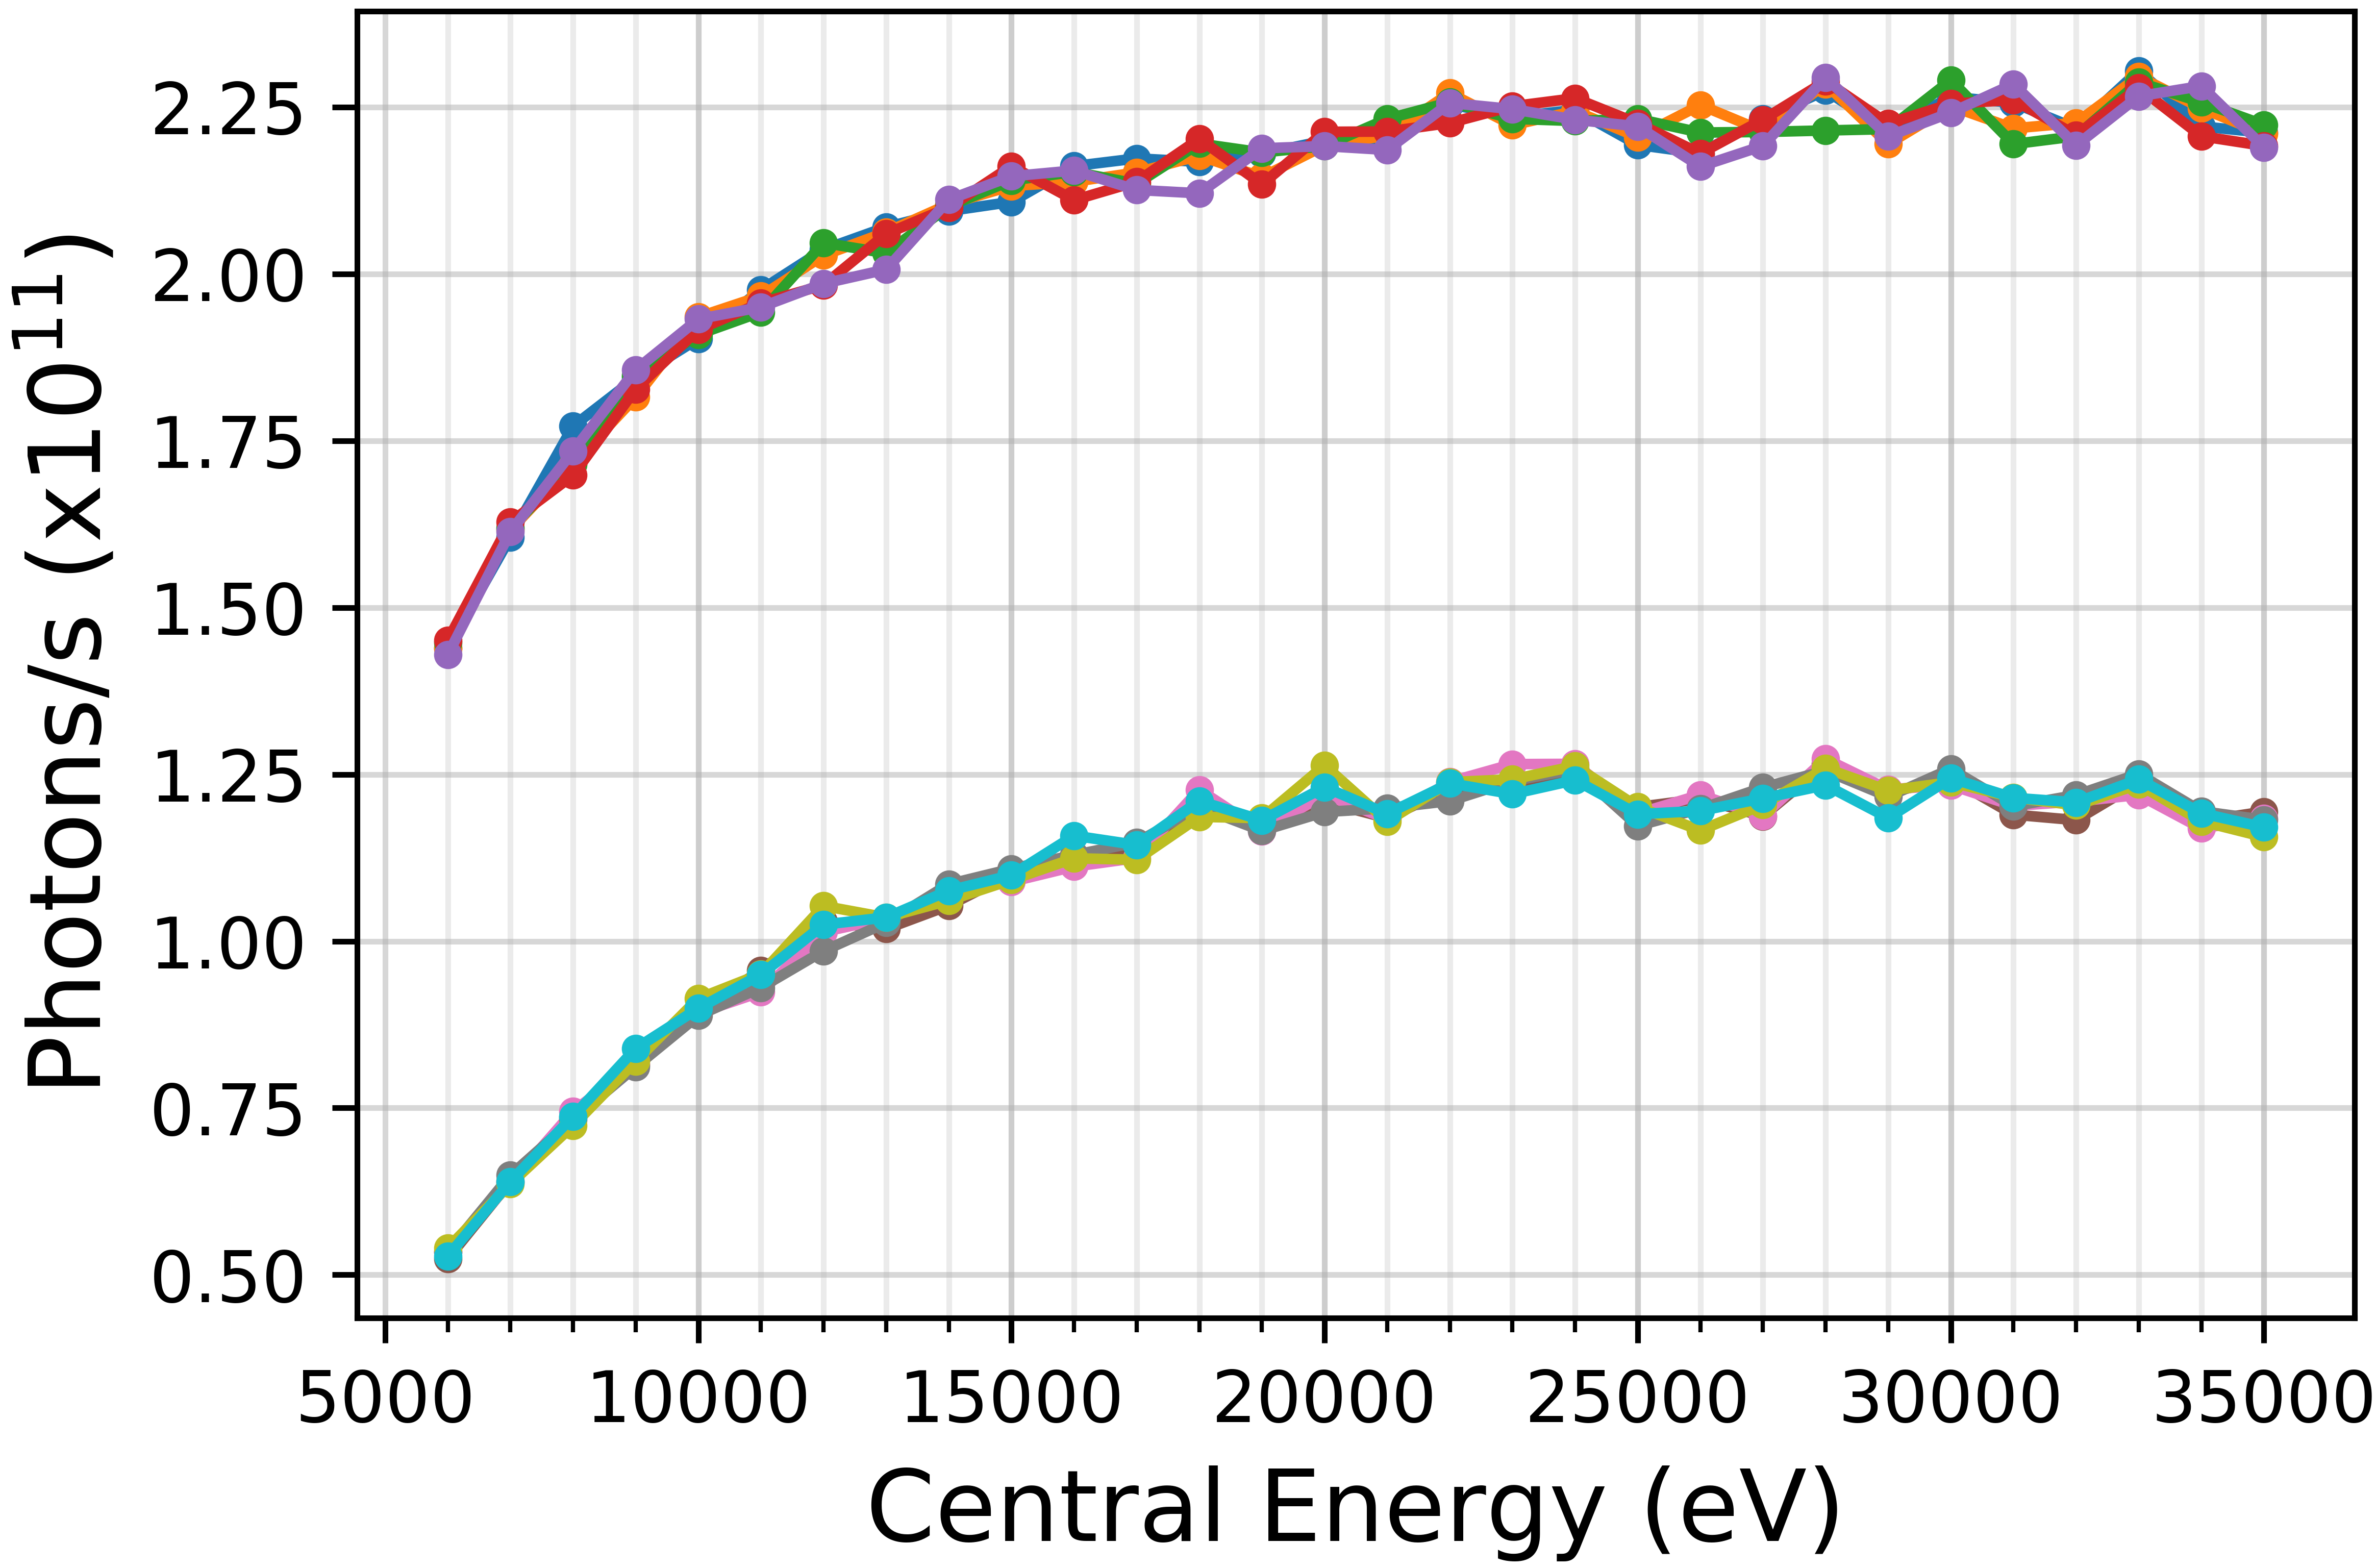
\includegraphics[width = 8.85cm]{images/333strainsize.png}
\label{fig:333strainsourcesize}
\end{figure}

\begin{figure}
\caption{Double crystal photon flux in Si~111 for strained and unstrained cases using an undulator source with parameters given in Table~\ref{ivubiomax}.}.
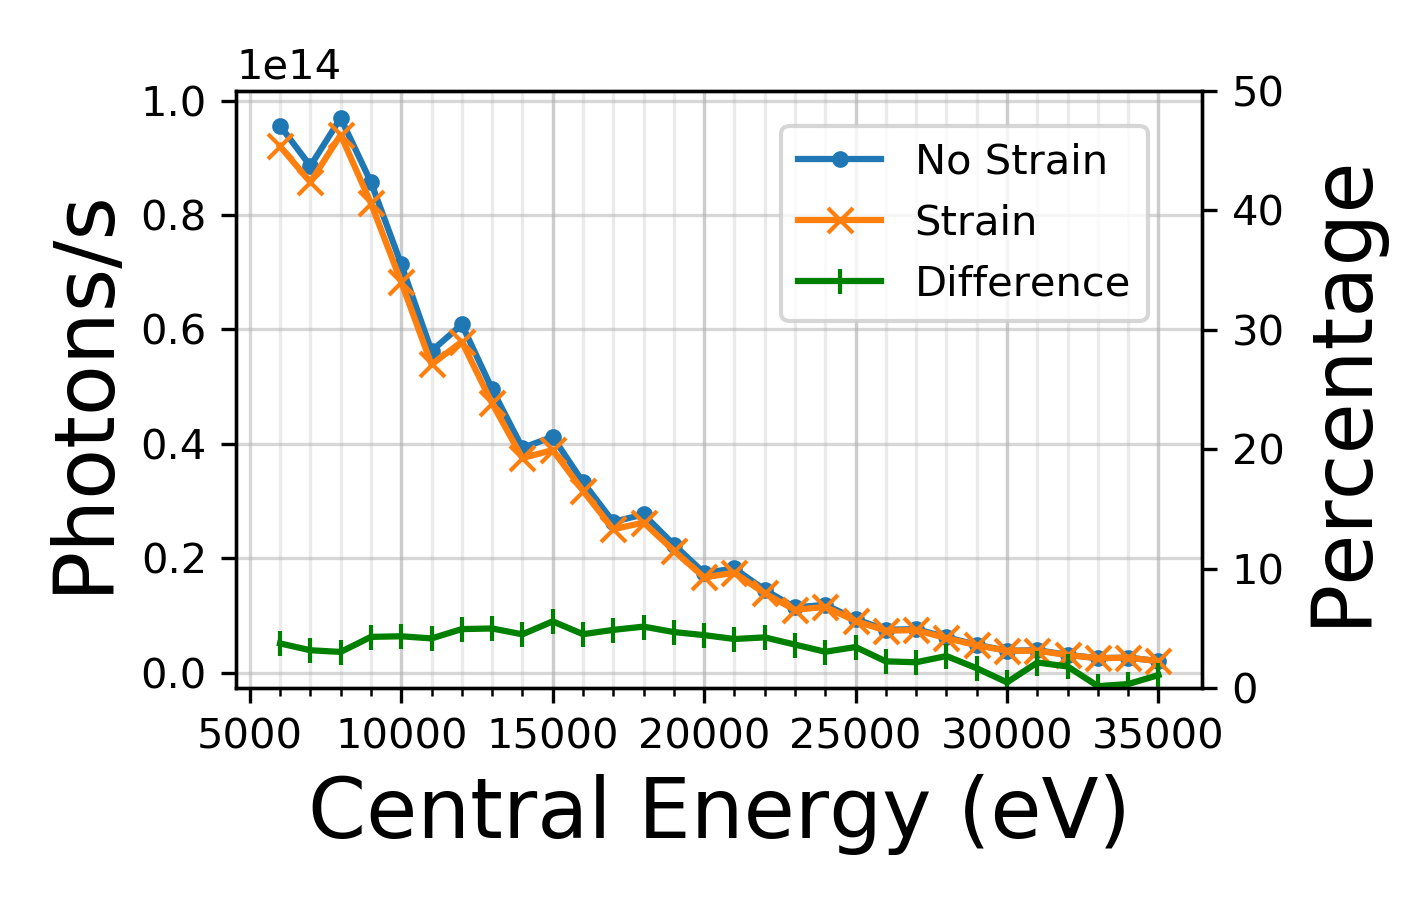
\includegraphics[width = 8.85cm]{images/ivu111flux.png}
\label{fig:ivu111flux}
\end{figure}

\begin{figure}
\caption{Double crystal photon flux in Si~333 for strained and unstrained cases using an undulator source with parameters given in Table~\ref{ivubiomax}.}
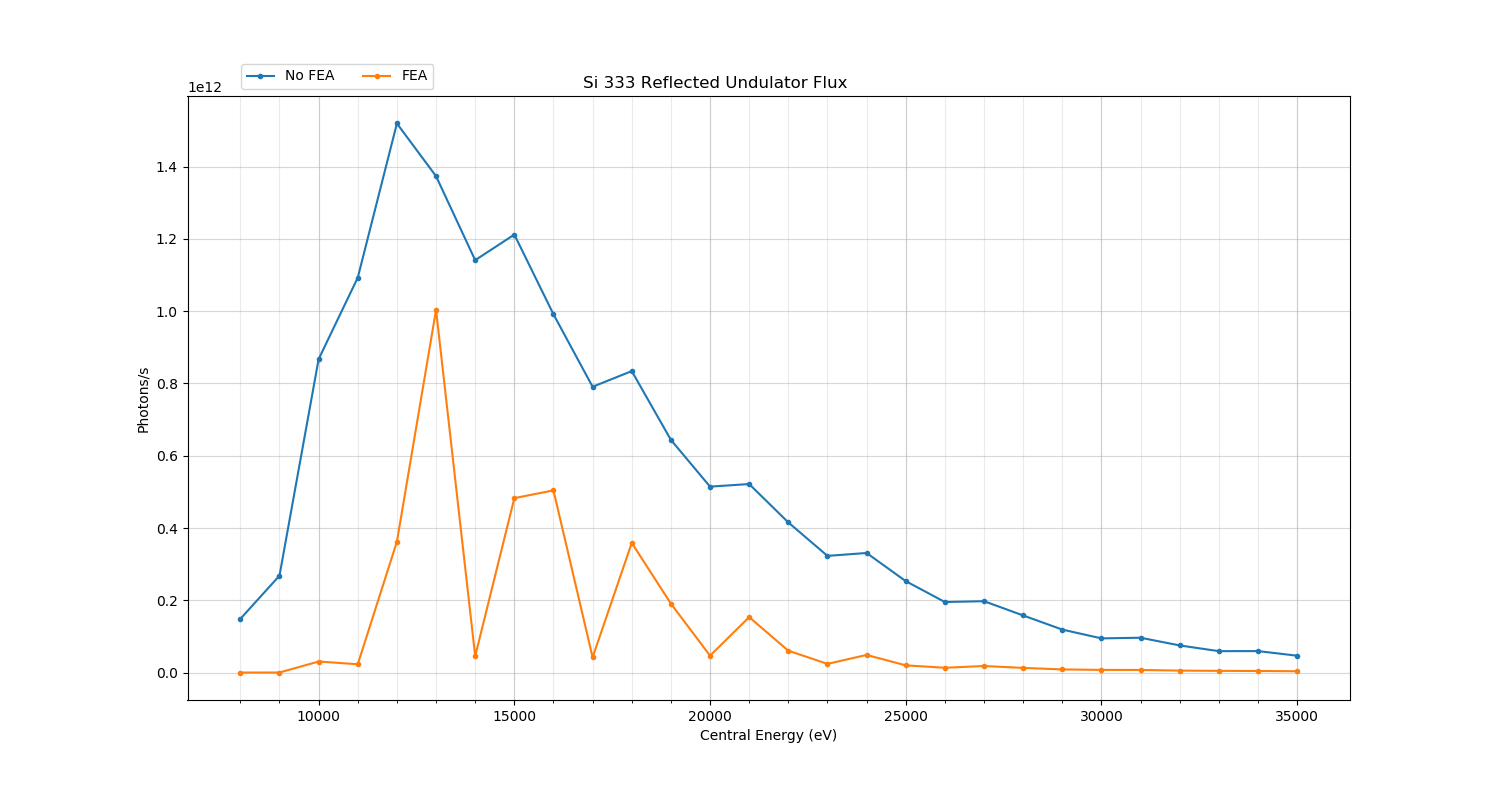
\includegraphics[width = 8.85cm]{images/ivu333flux.png}
\label{fig:ivu333flux}
\end{figure}

\begin{figure}
\caption{Double crystal photon flux in Si~333 at 22~keV for unstrained case as well as strained cases for second crystal tweaking angles stated by the legend in degrees. Undulator source used with parameters given in Table~\ref{ivubiomax}.}
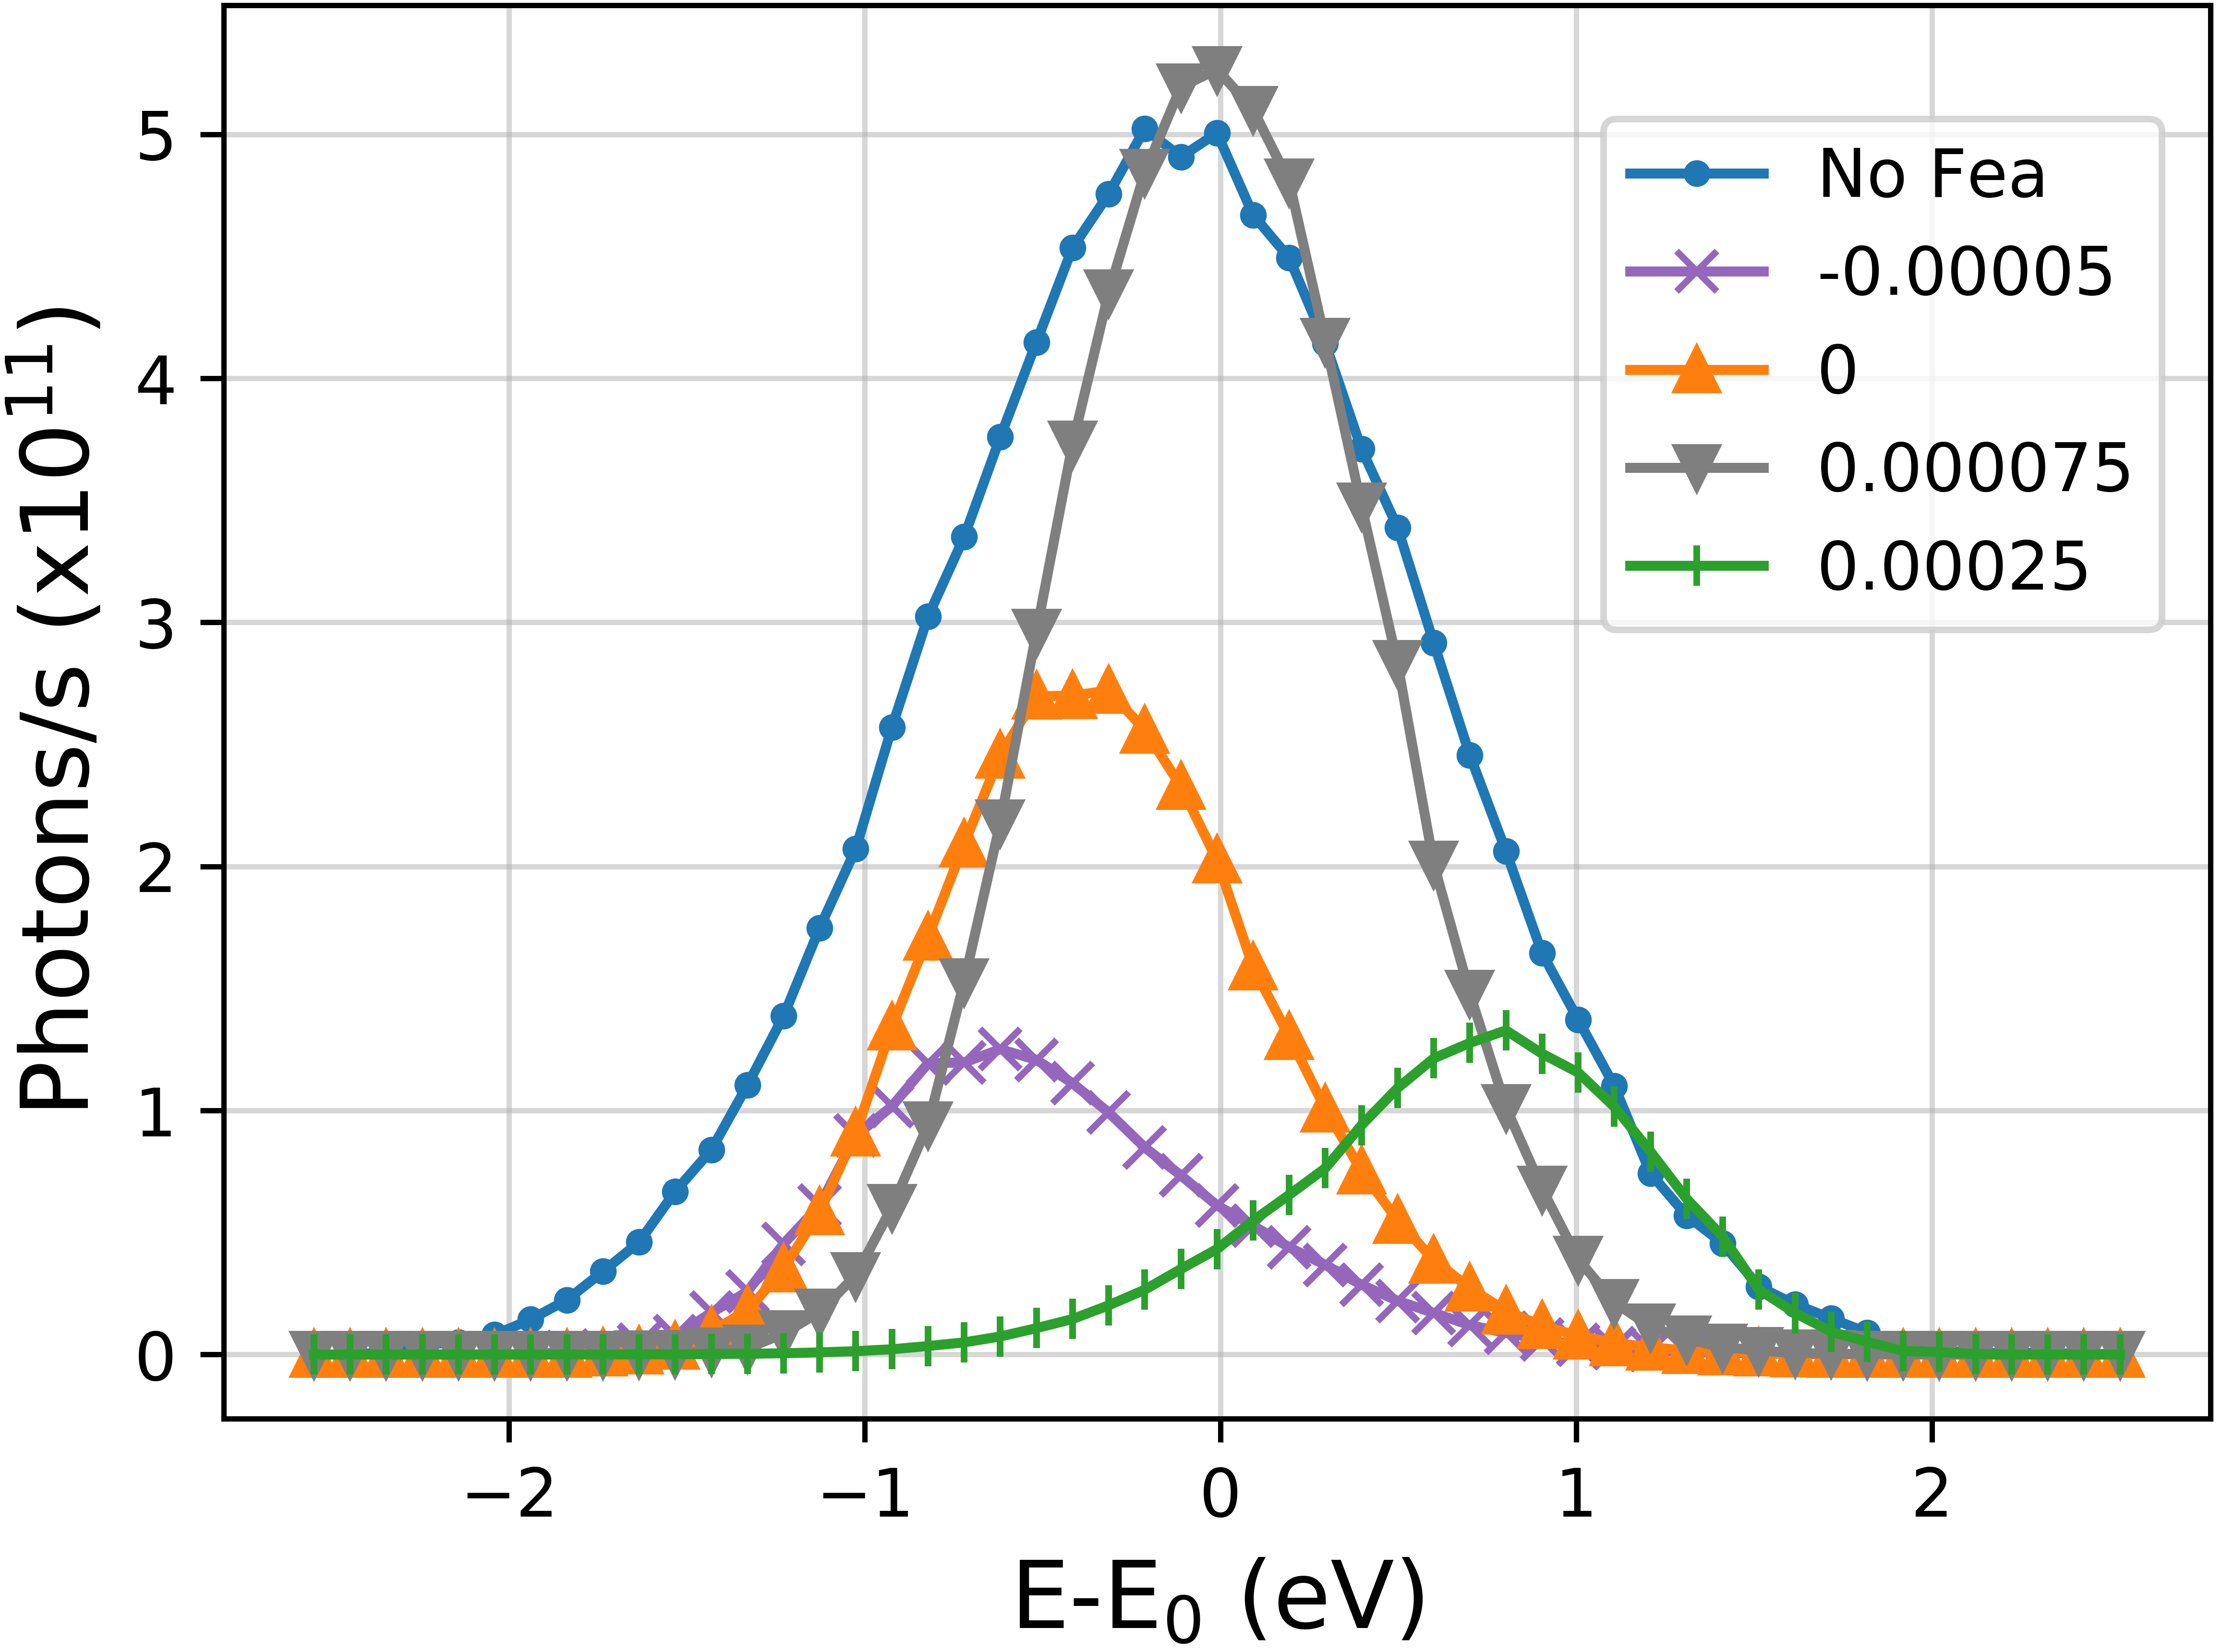
\includegraphics[width = 8.85cm]{images/26kevangle.png}
\label{fig:26kevangle}
\end{figure}

\begin{figure}
\caption{Double crystal photon flux in Si~333 unstrained and strained cases as well as case for maximum optimization angle of second crystal. Undulator source used with parameters given in Table~\ref{ivubiomax}.}
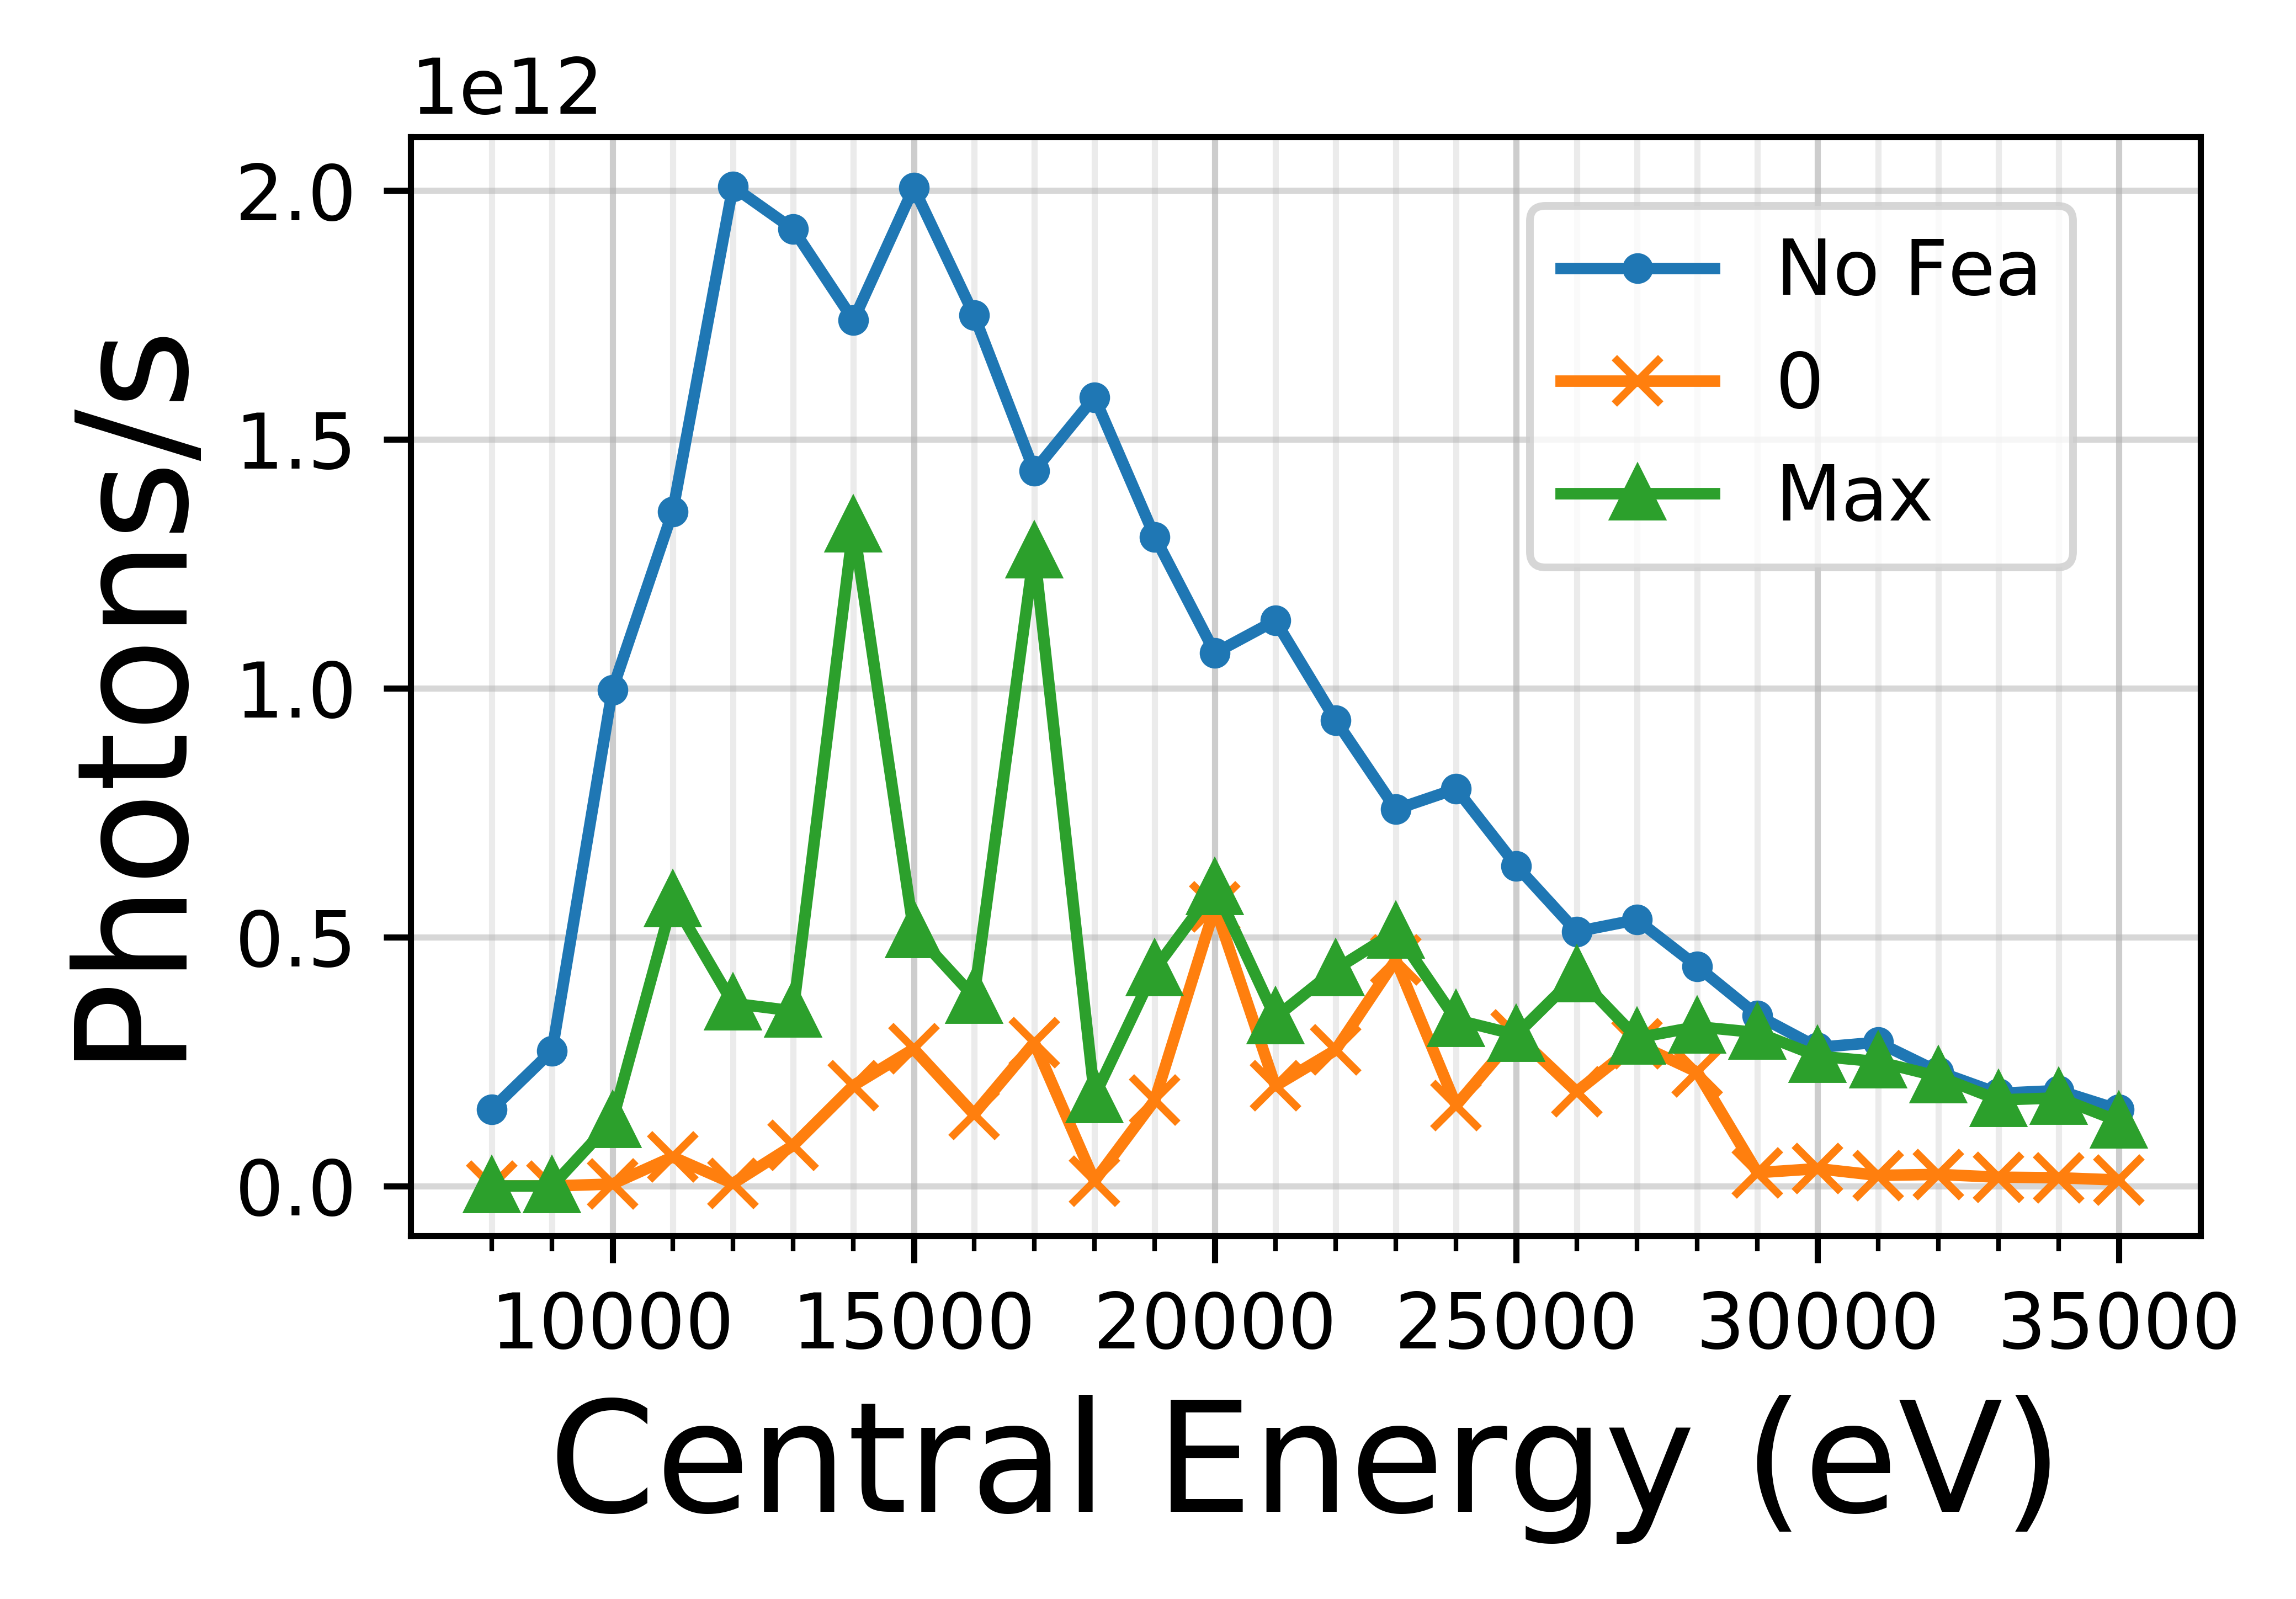
\includegraphics[width = 8.85cm]{images/maxangleflux.png}
\label{fig:maxangleflux}
\end{figure}

\begin{figure}
\caption{Double crystal photon flux in Si~111 for wiggler source for unstrained and strained cases. Difference in photon flux is also plotted.}
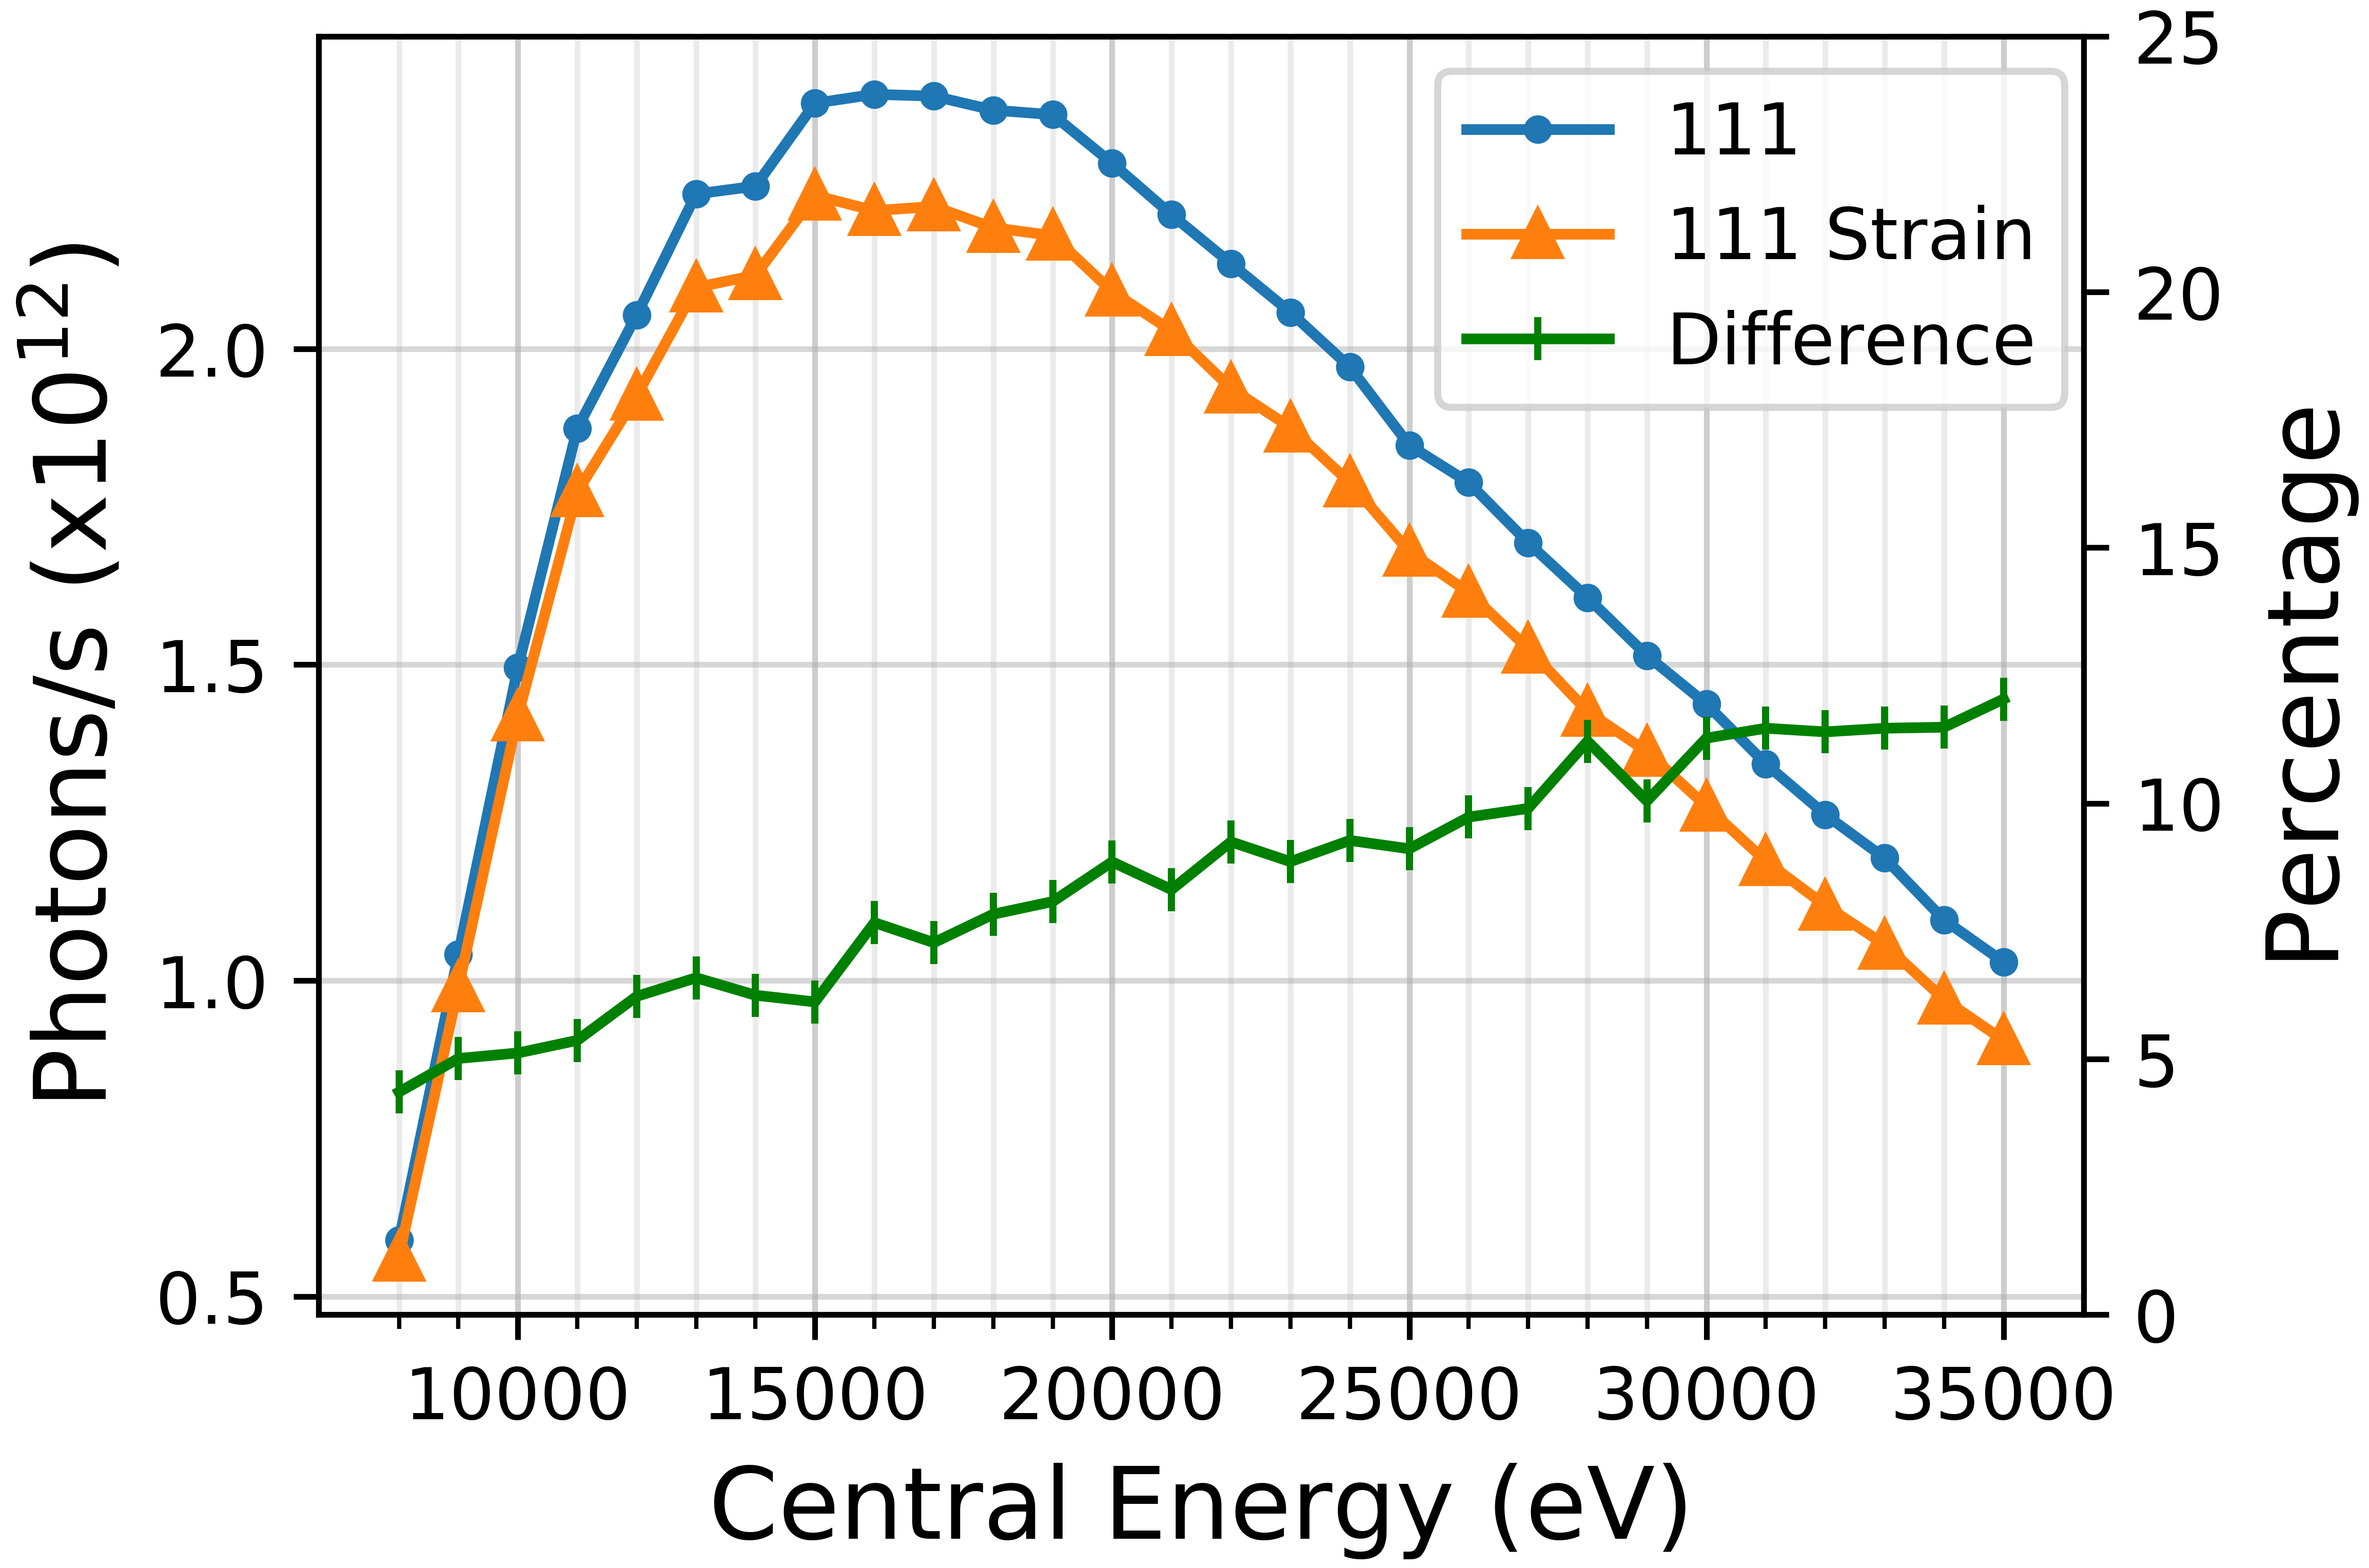
\includegraphics[width = 8.85cm]{images/ivw111flux.png}
\label{fig:ivw111flux}
\end{figure}

\begin{figure}
\caption{Double crystal photon flux in Si~311 for wiggler source for unstrained and strained cases. Difference in photon flux is also plotted.}
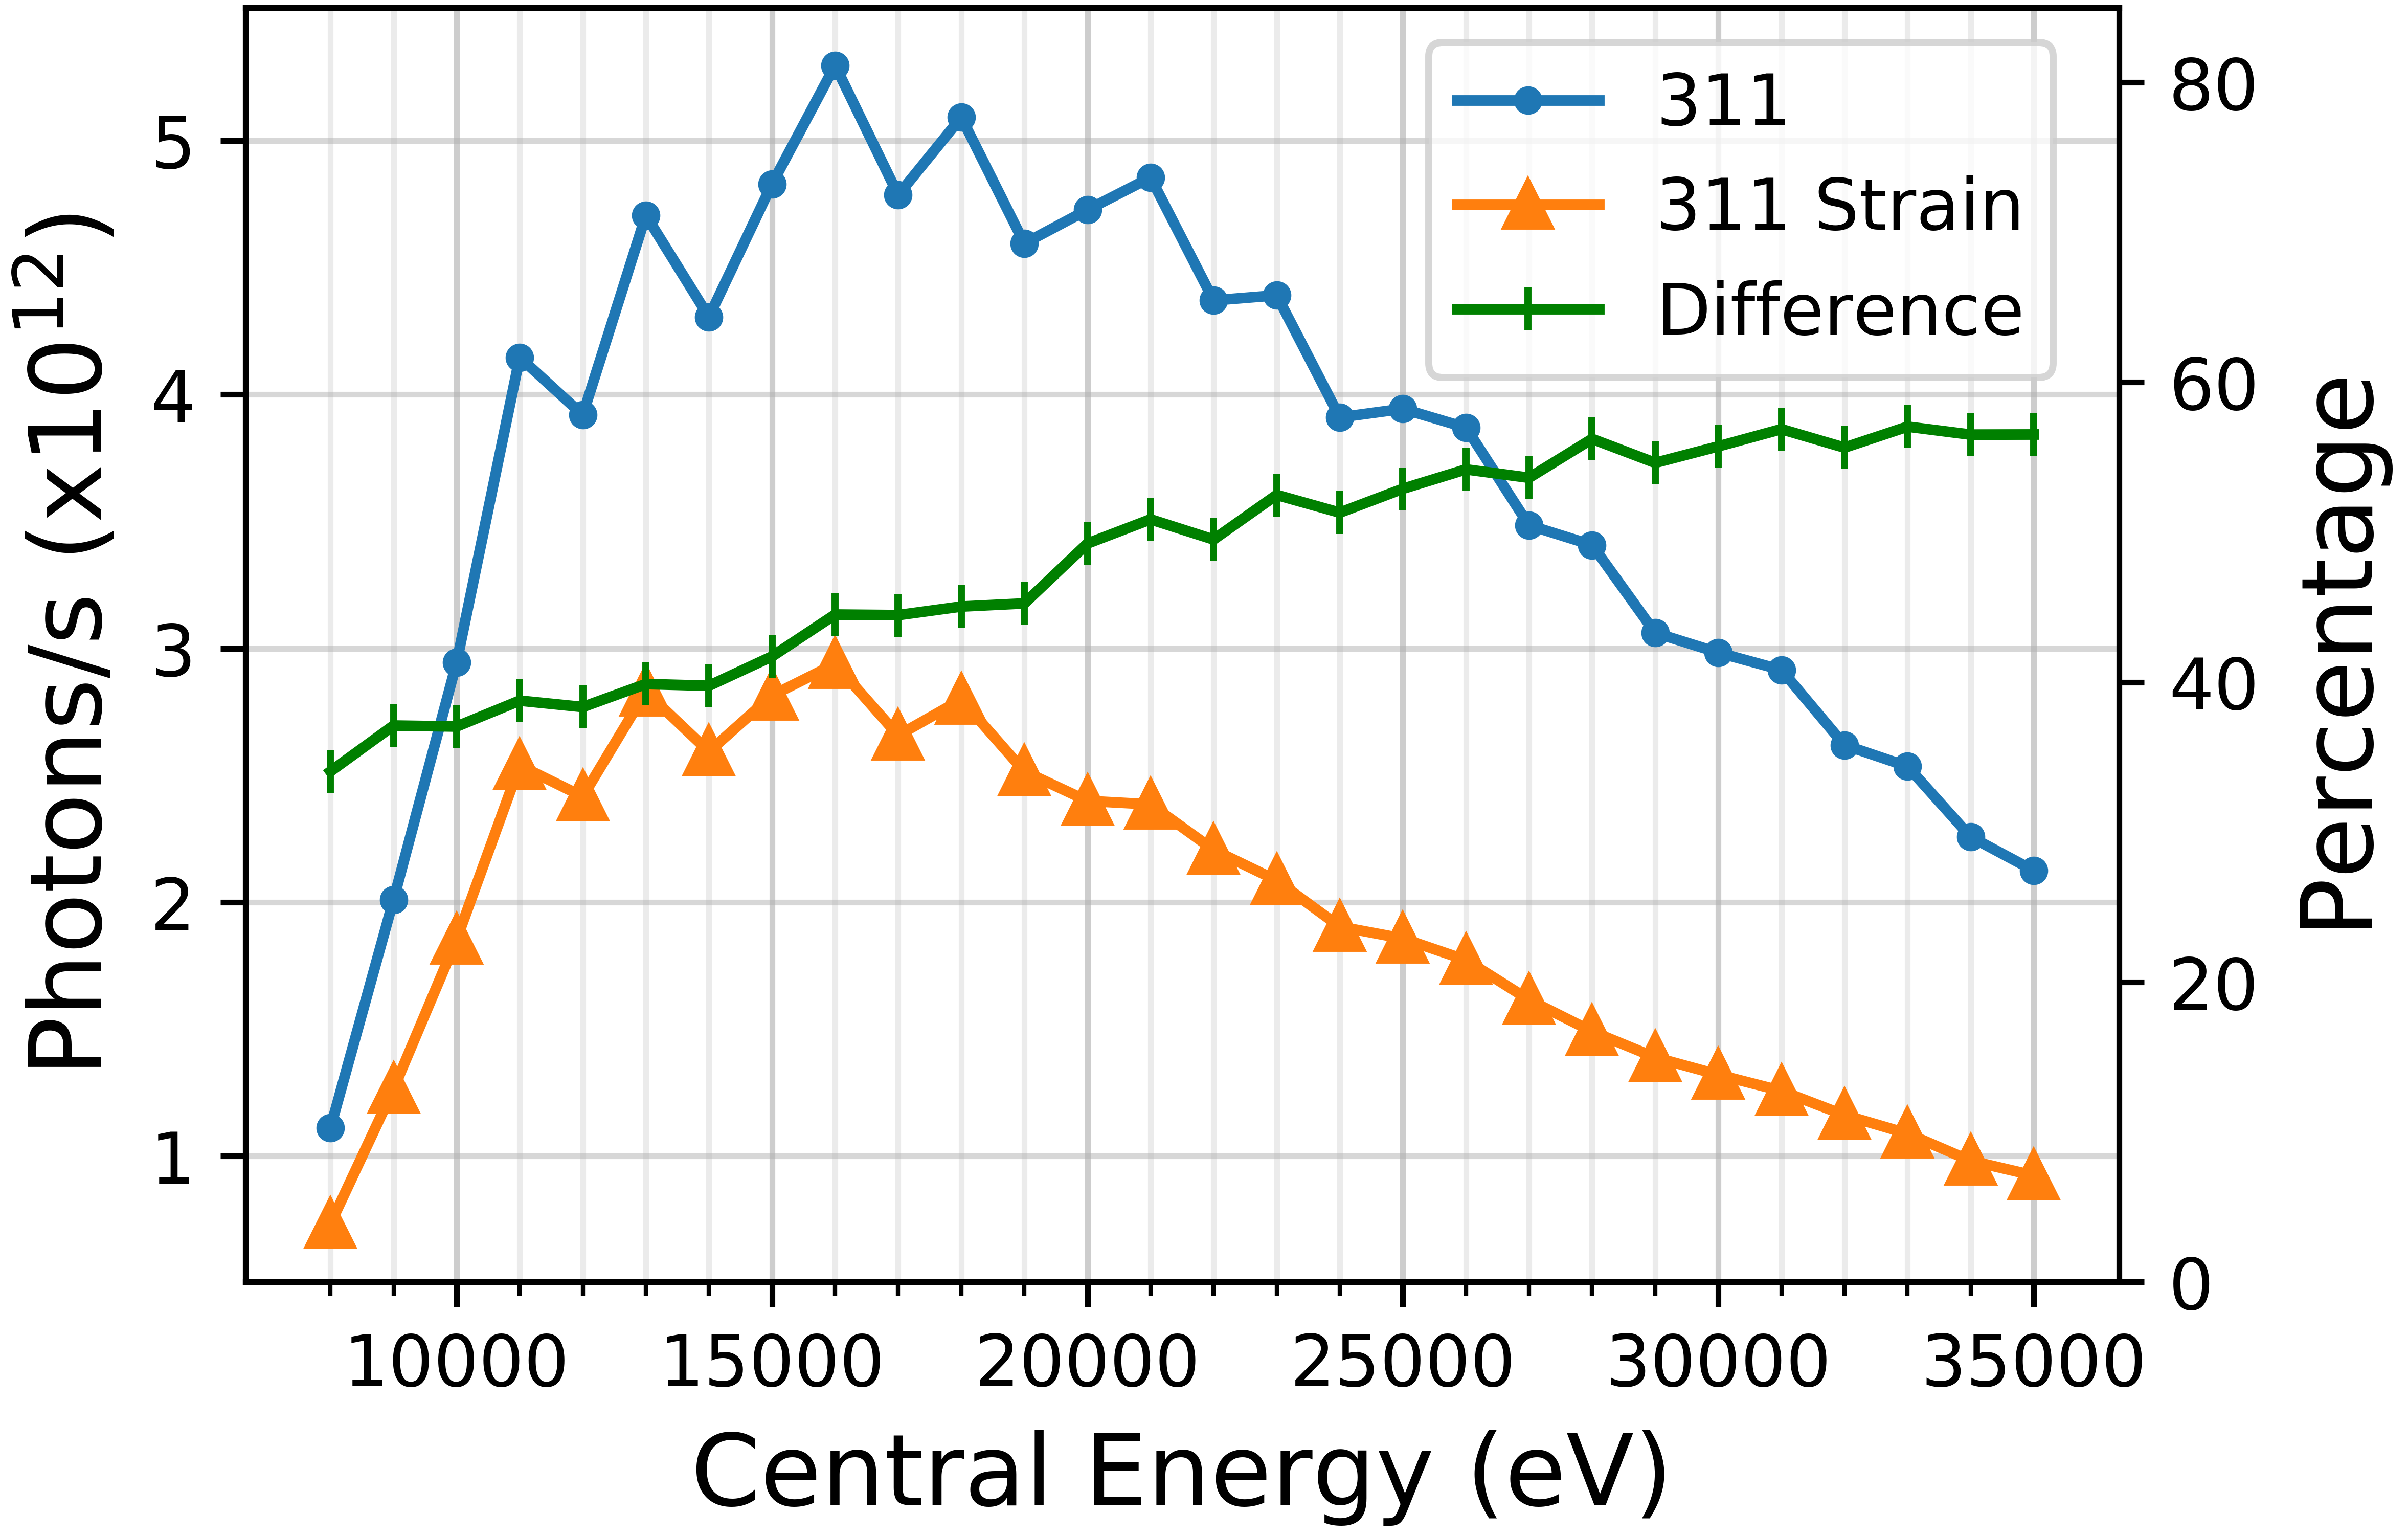
\includegraphics[width = 8.85cm]{images/ivw311flux.png}
\label{fig:ivw311flux}
\end{figure}

\begin{figure}
\caption{Double crystal photon flux in Si~333 for wiggler source for unstrained and strained cases with difference plotted. Also included is the maximum flux recovery due to second crystal angle adjustment.}
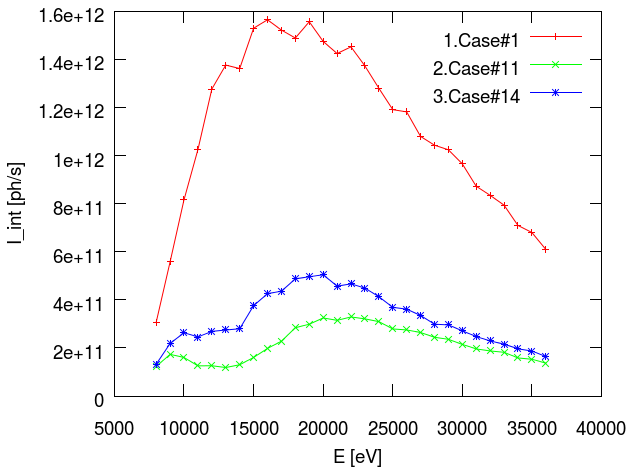
\includegraphics[width = 8.85cm]{images/ivw333flux.png}
\label{fig:ivw333flux}
\end{figure}

\begin{table}

\caption{Bare Silicon FEA Parameters}
\begin{tabular}{@{}llll@{}}
Parameter   & Value                   & Units                     & Description                        \\
\hline
$h$         & 0.3                     & W/(cm$^2\cdot$K)          & Heat transfer coefficient          \\
$T_{cool}$  & 77                      & K                         & Side cooling temperature           \\
$C_{11}$    & $1.6772\times 10^{11}$  & Pa                        & Stiffness tensor 11 component      \\
$C_{12}$    & $6.4980\times 10^{10}$  & Pa                        & Stiffness tensor 12 component      \\
$C_{44}$    & $8.0360\times 10^{10}$  & Pa                        & Stiffness tensor 44 component      \\
$C_p$       & 0.2                     & J/(g$\cdot$K)               & Heat capacity at constant pressure \\
$\rho$      &  2329                   & kg/m$^3$                  & Density                            \\
\end{tabular}
\label{baresiliconFEA}
\end{table}

\begin{table}

\caption{SSRL Silicon FEA Parameters}
\begin{tabular}{@{}llll@{}}
Parameter   & Value                   & Units                     & Description                        \\
\hline
$h$         & 1                       & W/(cm$^2\cdot$K)          & Heat transfer coefficient          \\
$T_{cool}$  & 77                      & K                         & Liquid Nitrogen Temperature        \\
$C_{11}$    & $1.6772\times 10^{11}$  & Pa                        & Stiffness tensor 11 component      \\
$C_{12}$    & $6.4980\times 10^{10}$  & Pa                        & Stiffness tensor 12 component      \\
$C_{44}$    & $8.0360\times 10^{10}$  & Pa                        & Stiffness tensor 44 component      \\
$C_p$       & 0.2                     & J/(g$\cdot$K)             & Heat capacity at constant pressure \\
$\rho$      &  2329                   & kg/m$^3$                  & Density                            \\
\end{tabular}
\label{ssrlsiliconFEA}
\end{table}

\begin{table}

\caption{Copper FEA Parameters}
\begin{tabular}{@{}llll@{}}
Parameter    & Value                  & Units                      & Description                        \\
\hline
$C_p$        & 385                    & J/(kg$\cdot$K)               & Heat capacity at constant pressure \\
$\kappa$     & 400                    & W/(m$\cdot$K)                & Thermal conductivity               \\ 
$\rho$       & 8960                   & kg/m$^3$                   & Density                            \\
\end{tabular}
\label{copperFEA}
\end{table}

\begin{table}
\caption{Indium FEA Parameters}
\begin{tabular}{@{}llll@{}}
Parameter    & Value                  & Units                      & Description                        \\
\hline
$C_p$        & 233                    & J/(kg$\cdot$K)               & Heat capacity at constant pressure \\
$\kappa$     & 81.6                   & W/(m$\cdot$K)                & Thermal conductivity               \\
$\rho$       & 7290                   & kg/m$^3$                   & Density                            \\
\end{tabular}
\label{indiumFEA}
\end{table}

\begin{table}
\caption{Liquid Nitrogen FEA Parameters}
\begin{tabular}{@{}llll@{}}
Parameter    & Value                  & Units                       & Description                        \\
\hline
$\mu$        & $157.9\times 10^{-6}$  & Pa$\cdot$s                  & Dynamic viscosity                  \\ 
$\gamma$     & 1.47                   & 1				            & Ratio of specific heats            \\
$C_p$        & 2.04                   & kJ/(kg$\cdot$K)               & Heat capacity at constant pressure \\
$\kappa$     & 139.6                  & mW/(m$\cdot$K)                & Thermal conductivity               \\
$\rho$       & 0.807                  & g/ml                        & Density                            \\
\end{tabular}
\label{nitrogenFEA}
\end{table}

\end{document}                    % DO NOT DELETE THIS LINE
%%%%%%%%%%%%%%%%%%%%%%%%%%%%%%%%%%%%%%%%%%%%%%%%%%%%%%%%%%%%%%%%%%%%%%%%%%%%%%